 
\documentclass[12pt]{article}

%打中文需要以下packages
\usepackage{xeCJK} 
\setCJKmainfont[BoldFont={cwTeXHeiBold}, ItalicFont={FandolSong}]{cwTeXMing} %Overleaf 中文字型設定
%\setCJKmainfont[BoldFont={cwTeX Q HeiZH}, ItalicFont={新細明體}]{cwTeX Q Ming}	
\XeTeXlinebreaklocale "zh"
\XeTeXlinebreakskip = 0pt plus 1pt %這兩行一定要加,中文才能自動換行


\usepackage{amssymb}
\usepackage{graphicx}
\usepackage{amsmath}
\usepackage[counterclockwise]{rotating}
\usepackage[hidelinks]{hyperref}
%\hypersetup{colorlinks,urlcolor=blue}
\hypersetup{colorlinks=true,citecolor=blue,pdfborder=000, urlcolor=red}
\usepackage{graphicx} % support the \includegraphics command and options
\usepackage[para,online,flushleft]{threeparttable}
\usepackage[round,semicolon]{natbib}  % This is for reference
\usepackage{cite}  % This is for reference
\usepackage{longtable}
%\usepackage{pdflscape}
\usepackage{rotating}
\usepackage{fancyhdr} % This should be set AFTER setting up the page geometry
\usepackage{epstopdf}
\usepackage{tikz}
\usepackage{caption}
\usepackage{subcaption}
%\usepackage{natbib} %This code is for Mac
\usepackage{booktabs} % for much better looking tables
\usepackage{array} % for better arrays (eg matrices) in maths
%\usepackage{paralist} % very flexible & customisable lists (eg. enumerate/itemize, etc.)
\usepackage{verbatim} % adds environment for commenting out blocks of text & for better verbatim
%\usepackage{subfig} % make it possible to include more than one captioned figure/table in a single float
% These packages are all incorporated in the memoir class to one degree or another...
\renewcommand{\arraystretch}{1.0} % 將表格行間距加大為原來的 1.2 倍
%%% HEADERS & FOOTERS
\usepackage{fancyhdr} % This should be set AFTER setting up the page geometry
%\pagestyle{fancy} % options: empty , plain , fancy
\usepackage{float} % 可固定表的位置
\usepackage{lscape}
\usepackage{bookmark} % Allow customized pdf bookmark
\usepackage{tabularx}

\setcounter{MaxMatrixCols}{12}

\renewcommand{\baselinestretch}{1.0}
\usepackage{indentfirst}
\usepackage{setspace,caption}
\captionsetup{font=doublespacing}% Double-spaced float captions
\doublespacing% Double-spaced document text

\setlength{\topmargin}{-0.5in}
\setlength{\textheight}{8.8in}
\setlength{\evensidemargin}{0.0in}
\setlength{\oddsidemargin}{0.0in}
\setlength{\textwidth}{6.5in}
%\input{tcilatex}

%%%%%%%  Change to Times New Roman format
\usepackage[tmargin=1in,bmargin=1in,lmargin=1in,rmargin=1in]{geometry}
%\usepackage{fontspec}
%\usepackage{xcolor}
\usepackage{titlesec}
%\defaultfontfeatures{Ligatures=TeX}
% Set sans serif font to Arial
%\setsansfont{Arial}
% Set serifed font to Times New Roman
%\setmainfont{Times New Roman}
% Set formats for each heading level
\titleformat*{\section}{\fontsize{16}{18}\bfseries\sffamily}
\titleformat*{\subsection}{\fontsize{14}{16}\bfseries\sffamily}
\titleformat*{\subsubsection}{\fontsize{12}{14}\bfseries\sffamily}

\newcommand{\bm}[1]{\boldsymbol{#1}}
\definecolor{cadmiumgreen}{rgb}{0.0, 0.42, 0.24}
\newcommand{\remarks}[1]{{\bf\color{cadmiumgreen}[#1]}}
\newcommand{\commentout}[0]{}

% 修改表格和圖片的標籤名稱
\renewcommand{\tablename}{表}
\renewcommand{\figurename}{圖}
\renewcommand{\abstractname}{摘要} % 手動修改摘要標題

% https://github.com/HungChunLi/ResearchMethodology-DSE

\usepackage{tabularx}

% \usepackage{datatool}
\usepackage{csvsimple}
\usepackage{booktabs} % 可選,用於美化表格

\begin{document}
	
	\title{\Large 初探台灣飲料市場需求體系}
	
	\author{\normalsize 黎宏濬\thanks{National Taiwan University, Email: r11627065@ntu.edu.tw}, 張立宏\thanks{National Taiwan University, Email: r11627065@ntu.edu.tw.},  林孝儒\thanks{National Taiwan University, Email: r11627065@ntu.edu.tw.},  許震浩\thanks{National Taiwan University, Email: r12323052@ntu.edu.tw.} \medskip}
	%{\normalsize \textbf{Job Market Paper 2}}}
	
	
	\maketitle
	
\begin{abstract}
This paper investigates the long-term effects of job displacement on earnings and mental health using administrative health claims data from Taiwan. Focusing on job loss resulting from mass layoffs, our estimates suggest a displaced worker experienced a 40\% decline in employment rates and a 67\% earning loss in the year following a layoff. Even after ten years, employment and earnings do not fully recover. Displaced workers also experience a deterioration in mental health, particularly related to stress, with a 16\% increase in outpatient visits for mental health issues and a 57\% increase in medical costs for mental illness. The negative impact on mental health is more pronounced among workers with lower earnings, men, and older individuals.
	
\end{abstract}


\newpage




%https://conversableeconomist.blogspot.com/2020/02/writing-intro-to-your-economics.html
\section{前言}

\subsection{研究背景}

隨著健康意識的逐漸提升,飲料市場的需求格局正在發生顯著變化。台灣作為一個消費者多樣化的市場,飲料需求受價格、收入及健康相關因素影響的特性具有研究價值。本研究以台灣飲料市場為例,探討消費者行為與需求系統的關聯,尤其關注健康意識的增強對不同飲料類別需求的影響。
過去的相關研究為本研究提供了堅實的理論基礎。\citet{RN2} 以「近似理想需求系統」(AIDS)模型分析美國市場不同飲料的需求彈性,發現非碳酸飲料具有奢侈品屬性,而咖啡與茶則被視為必需品。
\citet{RN1} 採用 LA/QUAIDS 模型分析日本市場,揭示了消費者年齡層與季節性變化對飲料需求的顯著影響。
同時,\citet{RN9} 指出,飲料製造商正響應健康需求,減少糖、鈉等成分,並引入健康標籤來吸引消費者。
此外,\citet{RN15} 強調了健康認知與媒體資訊在推動功能性飲料需求中的核心作用。

\subsection{研究目的}

為進一步驗證健康意識對台灣飲料市場的影響,本研究基於台灣經濟部工業產銷存動態調查資料庫及勞動部勞動統計查詢網,蒐集了1982年至2024年間五大飲料類別(果蔬汁飲料、碳酸飲料、運動飲料、咖啡飲料及茶類飲料)的月度銷售數據及收入數據。透過 AIDS 和 LA/AIDS 模型的應用,我們將探索健康意識提升如何影響台灣市場無糖與低糖飲料的需求,並評估價格與支出變化對飲料需求的影響特徵。
本研究期望填補台灣飲料市場健康需求相關研究的空白,為產業策略規劃與政策制定提供實證支持。

\section{文獻回顧}

在探討台灣飲料市場的需求系統時,我們主要聚焦於消費者健康意識的增強,以及不同產品價格對於消費者偏好的影響。針對美國飲料市場,\citet{RN2} 的研究運用「近似理想需求系統」(AIDS)模型分析了不同飲料的需求彈性,揭示了各類產品在奢侈性和必需性上的特徵。研究發現,非碳酸飲料的支出彈性較高,因此被視為奢侈品,而咖啡和茶則顯示其作為必需品的屬性。這表明,消費者在價格和支出上對不同飲料的需求具有顯著的敏感性差異。

\citet{RN1} 在日本市場的研究中,運用了 LA/QUAIDS 模型,分析健康標籤和功能性成分對消費者偏好的影響。該研究指出,不同年齡層的消費者對飲料的偏好存在顯著差異:年輕人更傾向於選擇果汁和牛奶,而老年人則偏好茶飲。此外,溫度對飲料需求的影響也十分顯著,隨著氣溫上升,冷飲的需求增加,而熱飲需求則有所下降。這些結果展示了人口統計因素與季節性變化在需求系統中的重要性,對於理解台灣市場中不同飲料在不同氣候條件下的需求特徵具有參考價值。

\citet{RN9} 的研究表明,飲料製造商正逐步響應消費者對健康產品需求的變化,通過減少產品中的糖、鈉及人工甜味劑,並引入「低糖」、「低鈉」等健康標籤來吸引消費者。與此同時,\citet{RN3} 的文獻回顧聚焦於歐洲地區軟性飲料(soft drinks)的消費模式,結合各國代表性飲食調查數據,探討了健康意識增強、政策干預及人口結構對飲料需求的影響。這些研究為健康政策的制定及市場需求的精準分析提供了實證支持。

此外,\citet{Rn15} 提出了一個全面的消費行為模型,揭示了健康認知、社會影響和媒體資訊在驅動功能性飲料需求中的核心作用。該研究指出,消費者在面臨健康威脅時,對具有增強免疫力、抗氧化或促進整體健康功能的飲料表現出更高的需求彈性。

隨著消費者對含糖飲料(SSBs)健康風險的認知不斷加深,市場對低糖或無糖飲料的需求也呈現出顯著的增長趨勢,尤其在青少年和老年消費者群體中更為明顯\citep{RN3}。隨著健康意識的普及,飲料行業逐步向生產更健康的產品轉型,我們希望通過需求系統模型驗證這一趨勢是否同樣適用於台灣市場,並進一步探索台灣消費者對無糖和低糖飲料需求的潛在增長,以評估健康意識增強對需求的具體影響。
 

% \section{資料與敘述統計}\label{data}

% \subsection{資料}
% Our study employs administrative data acquired from Taiwan's Health and Welfare Data Science Center (HWDC) to carry out the empirical analysis. We specifically make use of four distinct data sources from the HWDC: (1) National Health Insurance (NHI) enrollment records; (2) NHI claim files for outpatient care; (3) NHI claim files for inpatient care. To connect individuals across these data sources, we utilize their scrambled national identification numbers.


% \subsection{敘述統計}\label{em_strategy}
% Our sample comprises individuals aged 20-65 who were employed in a firm with at least 5 employees in the baseline year. We define displaced workers, our treatment group, as those who were employed for a minimum of five years prior to losing their jobs and underwent a mass layoff in a given year between 2005 and 2007. A mass layoff is characterized by a firm reducing its employment by over 90\% compared to the previous year. We track these workers for 16 years, including five years before and ten years after job loss. The control group consisted of non-displaced workers who had continuous employment during the sample period and worked in stable firms, which had no more than a 30\% employment decrease in December year-on-year.\footnote{Note that they are not necessary to stay in the same firm.} Since many workers satisfy this criterion, we randomly select 10\% of them to serve as the control group. Our final sample is resulting in 9,700 workers from the treatment group and 332,720 from the control group.

% Our empirical strategy to identify the dynamic effects of displacement on earnings and mental health involves estimating the following regression:
% \begin{equation}\label{event}
% 	Y_{it}= \underset{k = -5}{\overset{10}{\sum }}\delta_{k} \cdot Disp_{i} \times \mathbf{I}[t=c+k] + \underset{k = -5}{\overset{10}{\sum }}\gamma_{k} \cdot \mathbf{I}[t=c+k] 
% 	+ \alpha_i 
% 	+ \pi_t
% 	+ X_{it} \beta
% 	+\varepsilon_{it}.
% \end{equation}
% $Y_{it}$ is the outcome of interest for worker $i$ in year $t$: 1) Employment (a dummy indicating working for at least one month per year or not); 2) Annual earnings; 3) Cumulative number of visits for mental illness; 4) Cumulative medical expenses of mental illness (including both outpatient and inpatient care).   $Disp_{i}$ indicates whether worker $i$ is a displaced worker. $I(t=c+k)$ is a dummy variable indicating $k$ years after (pseudo) mass layoff year, $c$, where $k$ does not include $-2$ since we consider two years prior to a job loss as the reference year.\footnote{For the comparison group, the pseudo mass layoff year is the year we use to confirm the firm did {\it not} go through a mass layoff and remain no more than 30\% reduction in the firm size.)} $\gamma_{k}$ represents the evolution of outcomes among non-displaced workers. $\delta_{k}$ is the coefficient of interest, which measures the change in outcomes among displaced workers with respect to the reference year ($k=-2$), relative to the change of non-displaced workers. We additionally control individual fixed effects ($\alpha_i$) and calendar year fixed effects ($\pi_t$). $X_{it}$ are other controls, mainly quartic function of worker's age and county/municipality level unemployment rate.

\section{資料蒐集與處理}
\subsection{資料蒐集}
本研究使用的資料主要來自於「經濟部工業產銷存動態調查資料庫」,涵蓋5種飲料類別(果蔬汁飲料、碳酸飲料、運動飲料、咖啡飲料及茶類飲料)的銷售量與銷售值的月資料,詳細記錄了每種飲料的市場表現。此外,另一部分資料來自於「勞動部勞動統計查詢網」的國民所得月度統計資料,用以反映消費者的收入水準。所有資料的涵蓋期間為1982年至2024年,共收集到547筆月統計資料,確保了樣本的時間跨度。這些數據不僅提供了每類飲料的銷售量和銷售值,也包含了與消費行為密切相關的消費者所得,為後續的DSE(Demand System Estimation)分析提供了關鍵依據。

\subsection{資料處理}
在完成資料蒐集後,我們按步驟進行了資料處理,目的是提高數據的可靠性與一致性。首先,我們使用 R 統計軟體對資料進行清理,包括合併不同來源的數據、去除重複資料、以及處理遺漏值等工作。對於部分遺漏值,考量到補值可能帶來的偏誤,我們選擇將無法合理填補的觀察值移除。此外,由於不同飲料類別的統計起始時間不一致,我們將分析的起始時間進行統一,確保資料具有可比性。為了進一步豐富研究變數,我們還根據銷售量與銷售值兩個變數計算並新增了每種飲料的單位價格,為我們後續使用模型估計去衡量價格對消費者需求的影響提供了必要的解釋變數。

\section{研究設計}

本文分別採用 AIDS (Almost Ideal Demand System)和 LA/AIDS (Linear Approximate AIDS) 兩種需求系統模型進行分析。
兩種方法皆用於分析多個商品的需求及其需求彈性,主要差別在於價格指數的處理方式,。
以下兩節將分別敘述 AIDS 及 LA/AIDS 的模型架構。

\subsection{使用AIDS模型分析}

\[
	w_i = \alpha_i + \sum_{j=1}^{5} \gamma_{ij} \ln(P_j) + \beta_i \ln\left(\frac{X}{P}\right),
\]
\begin{itemize}
	\item $w_i = \frac{P_i Q_i}{X}$: expenditure share of the $i$-th beverage category
	\begin{itemize}
		\item $P_i$ is the price of the $i$-th beverage
		\item $Q_i$ is the quantity of the $i$-th beverage
		\item $X$ is the total expenditure on all beverages, which may vary with monthly income
	\end{itemize}
	\item $\ln(P_j)$: The natural logarithm of the price of the $j$-th beverage
	\item $P$: Price index, typically approximated by the Stone price index:
	\begin{equation*}
	\ln(P) = \sum_{j=1}^{5} w_j \ln(P_j),
	\end{equation*}
	where $w_j$ is the expenditure share of the $j$-th beverage
	\item $\alpha_i$, $\gamma_{ij}$, $\beta_i$: Parameters to be estimated for each beverage category
\end{itemize}

\subsection{使用LAAIDS模型分析}


\section{AIDS及LAAIDS模型參數估計結果}

% \subsection{係數解釋}

% 表 \ref{coef} 記錄了AIDS與 LAAIDS模型的估計結果,其探討了果蔬汁、碳酸飲料、運動飲料、咖啡飲料及茶飲料的需求特徵。
% \texttt{alpha} 係數反映了收入不變時,各飲料的基礎需求水準。兩模型的結果一致指出,果蔬汁和咖啡飲料擁有較高的基礎需求。在AIDS 模型及LAAIDS 模型中,果蔬汁的\texttt{alpha 1}估計值分別為 1.24和 1.16;咖啡飲料的\texttt{alpha 4}估計值則為 0.69和 0.76,顯示這兩類飲料對消費者來說是穩定的日常選擇,特別是果蔬汁的健康屬性和咖啡飲料的功能性使其市場地位穩固。相較之下,碳酸飲料的基礎需求偏低,\texttt{alpha 2} 值分別為 0.54和 0.42,顯示健康意識的提升對其需求造成了一定影響,運動飲料的需求基礎有限,\texttt{alpha 3}值在兩模型中均為負(-0.30 和 -0.27),說明其消費群體較為特定,需求具有較高彈性。而茶飲料的\texttt{alpha 5}值為-1.17 和 -1.07,反映其基礎需求在市場中相對最低。

% beta 係數衡量總支出變化對需求的影響。\texttt{beta 1}(果蔬汁)的 beta 值在兩模型中均為負,顯示總支出增加時其需求略有下降,可能因為消費者轉向更高端飲品如運動飲料和茶飲料。\texttt{beta 3}(運動飲料)的值在兩模型中均為顯著正值,表明其需求隨總支出上升而增加。同樣,\texttt{beta 5}(茶飲料)的 beta 值亦為正,顯示總支出增加會促進需求增長,強化了其作為正常財的特性。\texttt{beta 2}(碳酸飲料)的值雖接近顯著性,但在兩模型中呈現出正值,表明總支出對其需求影響有限但可能略有促進。而\texttt{beta 4}(咖啡飲料)的值為負,顯示其需求會隨總支出提升而減少。

% gamma 係數揭示了飲料間的替代與互補關係。兩模型均表明,\texttt{gamma 5 4}(茶飲料與咖啡飲料)之間的替代效應較弱,當茶價格上升時,咖啡需求也會減少(gamma 值為負),可能反映了兩者目標消費群體的差異。\texttt{gamma 2 5}(碳酸飲料與茶飲料)之間的替代性較強,當茶價格上升時,碳酸飲料需求增加,表明碳酸飲料是茶的重要替代品。此外,果蔬汁與其他飲料的 gamma 值表現出一定的互補性。


\subsection{支出彈性}

% 表 \ref{exp} 記錄了 AIDS 和 LAAIDS 模型的支出彈性結果,探討果蔬汁、碳酸飲料、運動飲料、咖啡飲料及茶飲料在台灣市場的需求在面對總支出變動時的敏感性。

% 運動飲料在AIDS 模型和LAAIDS 模型中的支出彈性分別為 1.41與 1.38,為所有飲料類型中最高,顯示其需求對總支出變動極為敏感。茶飲料的支出彈性分別為 1.34與 1.32,隨著總支出的提升,茶飲料需求大幅增長。果蔬汁的支出彈性在兩模型中分別為 0.52和 0.55,顯示其需求對總支出變動不敏感,這表明果蔬汁的消費穩定,即使總支出波動,其需求變化幅度也較小。咖啡飲料的支出彈性在兩模型中分別為 0.54與 0.50,標示消費者對咖啡飲料的需求穩定。碳酸飲料的支出彈性在兩模型中分為 0.85與 0.91,接近 1,顯示其需求隨總支出的變化呈接近比例的增長。

表 \ref{exp} 記錄了 AIDS 和 LAAIDS 模型的支出彈性結果,探討台灣市場中五種飲料在總支出變動下的需求敏感性。

運動飲料的支出彈性在 AIDS 和 LAAIDS 模型中分別為 1.41 和 1.38,為最高,顯示對總支出變動最敏感。茶飲料彈性為 1.34 和 1.32,需求隨總支出顯著增長。果蔬汁彈性分別為 0.52 和 0.55,需求穩定,總支出變動影響有限。咖啡飲料彈性為 0.54 和 0.50,同樣顯示穩定需求。碳酸飲料彈性分別為 0.85 和 0.91,接近 1,表明需求與總支出呈比例增長。

\subsection{Marshallian 需求彈性}

% Marshallian 需求函數又稱為未補償需求函數(uncompensated demand function),描述的是在給定收入和價格條件下,消費者如何選擇商品組合以最大化效用,其考慮了包含收入在內的所有外生因素,因此顯示各飲料需求對於價格變動的總反應。從表 \ref{aids_marshall}和表\ref{laaids_marshall}可以看出對各種商品估計的 Marshallian 需求彈性,揭示其對自身與其他飲料價格變動的敏感性及市場定位。

% 果蔬汁在 AIDS 模型及 LAAIDS 模型中的自價格彈性分別為 -0.45 及 -0.04,顯示其需求穩定,碳酸飲料自價格彈性分別為 -0.59 及 -0.51 ,表明需求對價格波動較敏感,健康意識提升可能進一步影響其市場。運動飲料自價格彈性為 -0.27 及 -0.66 ,反映其需求在健康飲品市場中對價格有所敏感。咖啡飲料的自價格彈性為 0.37 及 0.84 ,可能反映品牌價值帶來的特殊消費行為。茶飲料自價格彈性在兩模型中分別為 -0.06  及 -0.35 ,顯示其需求對價格變動影響最小,具有高度穩定性。

% 在交叉價格彈性中,果蔬汁與碳酸飲料需求表現出一定的互補性,在 AIDS 模型及 LAAIDS 模型中分別為 -0.50 及 -0.42;而果蔬汁與運動飲料之間則顯示出顯著的替代效應,在兩模型中分別為 0.84 及 1.47。咖啡飲料與茶飲料之間的互補效應在兩模型中均顯著,在兩模型中分別為-1.82 及 -2.60,當茶價格上升時,咖啡需求顯著下降,顯示兩者在功能性消費中具有緊密聯動。

Marshallian 需求函數(未補償需求函數)描述消費者在給定收入與價格下的商品選擇,反映需求對價格變動的總反應。表 \ref{aids_marshall} 和表 \ref{laaids_marshall} 顯示了各飲料的需求彈性,揭示其對價格變動的敏感性及市場定位。

果蔬汁的自價格彈性在 AIDS 和 LAAIDS 模型中分別為 -0.45 和 -0.04,需求穩定;碳酸飲料為 -0.59 和 -0.51,需求對價格較敏感,可能受健康意識影響;運動飲料為 -0.27 和 -0.66,需求對價格有所敏感;咖啡飲料為 0.37 和 0.84,反映品牌價值的影響;茶飲料為 -0.06 和 -0.35,需求對價格變動影響最小,穩定性最高。

交叉價格彈性中,果蔬汁與碳酸飲料表現一定互補性(-0.50 和 -0.42);果蔬汁與運動飲料顯示顯著替代效應(0.84 和 1.47)。咖啡與茶的互補效應顯著(-1.82 和 -2.60),表明兩者在功能性消費中高度聯動。

\subsection{Hicksian 需求彈性}

% Hicksian 需求函數又稱為受補償需求函數(compensated demand function),描述的是在給定效用水準下,消費者如何選擇商品組合以最小化支出。在 Hicksian 需求中,需求彈性消除了收入效果,只考慮了替代效果。從表\ref{aids_hicks}和表\ref{aids_hicks}中可以看到 AIDS 和 LAAIDS 模型對各商品 Hicksian 需求彈性的估計結果。

% 在 AIDS 和 LAAIDS 模型中,碳酸飲料和運動飲料均表現出極高的需求彈性,碳酸飲料的自彈性分別為 -1.398 和 -1.466,而運動飲料的自彈性則為 -1.463 和 -1.307。這些數據顯示,這兩類飲料的需求對價格變動非常敏感,價格上升 1\% 會導致其支出占比顯著下降,表示消費者在價格波動時極易轉向其他替代商品。在 AIDS 模型中,果菜汁的價格彈性為 -0.354,而在 LAAIDS 模型中則為 0.069,表示果菜汁的需求對價格的敏感性相對較低。

% 茶飲料與碳酸飲料之間的替代效應最為強烈,當茶飲料價格上升 1\% 時,碳酸飲料的支出占比在 AIDS 模型中增加了 1.909,而在 LAAIDS 模型中增加了 1.806。同樣,茶飲料與運動飲料之間的替代效應也非常顯著,茶飲料價格每上升 1\%,運動飲料的支出占比增加 1.449 至 2.058。互補效應則在茶飲料與咖啡飲料之間顯得尤為顯著,當茶飲料價格上升 1\% 時,咖啡飲料的支出占比下降了 1.594 至 2.389,這表明消費者經常會同時購買這兩種飲料。

Hicksian 需求函數(受補償需求函數)描述消費者在給定效用水準下如何選擇商品以最小化支出,僅考慮替代效果。表 \ref{aids_hicks} 和表 \ref{laaids_hicks} 顯示了 AIDS 和 LAAIDS 模型的 Hicksian 需求彈性估計結果。

碳酸飲料和運動飲料表現出極高的自價格彈性(-1.398 和 -1.466;-1.463 和 -1.307),顯示其需求對價格極為敏感,價格上升 1\% 導致支出占比顯著下降。果菜汁價格彈性在 AIDS 模型中為 -0.354,在 LAAIDS 模型中為 0.069,需求對價格變動不敏感。

茶飲料與碳酸飲料的替代效應最強,茶價格上升 1\%,碳酸飲料支出占比在 AIDS 和 LAAIDS 模型中分別增加 1.909 和 1.806。茶飲料與運動飲料的替代效應也顯著,茶價格上升 1\% 時,運動飲料支出占比增加 1.449 至 2.058。茶與咖啡的互補效應尤為顯著,茶價格上升 1\% 導致咖啡支出占比下降 1.594 至 2.389,表明兩者經常被同時購買。


\subsection{}
We discuss a number of robustness checks for our main findings in Online Appendix \ref{dis_robust}, including different matching techniques, different estimation methods, and different choices of samples. In general, our main results are robust to these changes. Moreover, we conduct a set of subgroup analyses and discuss these results in the Online Appendix \ref{dis_hetero}. To sum up, our analysis suggests that the negative effect of job displacement on mental health appears to be more pronounced among lower-income workers, men, and older individuals.

\section{結論}\label{conclusion}

地區的限制性 Using Taiwan's administrative data, we examined the effects of job displacement on employment, earnings, and mental health. Due to the mandatory and generous nature of Taiwan's NHI, our study are less likely to suffer from sample attrition and to be confounded with changes in health insurance enrollment. On the other hand, the comprehensive NHI data allows us to explore the impact of displacement on both outpatient and inpatient healthcare use.



\newpage

% Your bibliography command here (e.g. \bibliography{your-bib-file}) if using natbib
% \bibliography{Job_loss_citation}{}
\bibliography{DSE_citation}{}
\bibliographystyle{chicago}

% \newpage

\section*{表格}

\newpage
\begin{table}[H]
    \caption{AIDS及LAAIDS模型估計結果與顯著性}
    \centering
    \begin{tabular}{cc} % 建立兩欄表格佈局
        % 左欄上方表格
        \begin{subtable}[t]{0.45\textwidth}
            % \centering
            \begin{center}
                \caption{Alpha參數} \label{coef_alpha}
                % latex table generated in R 4.3.1 by xtable 1.8-4 package
% Mon Nov 25 17:19:36 2024
\begin{tabular}{lll}
  \hline
變數 & (1) & (2) \\ 
  \hline
alpha 1 & 1.238*** & 1.164*** \\ 
   & (0.085) & (0.079) \\ 
  alpha 2 & 0.537*** & 0.418*** \\ 
   & (0.129) & (0.116) \\ 
  alpha 3 & -0.300*** & -0.269*** \\ 
   & (0.074) & (0.063) \\ 
  alpha 4 & 0.694*** & 0.760*** \\ 
   & (0.063) & (0.056) \\ 
  alpha 5 & -1.169*** & -1.073*** \\ 
   & (0.220) & (0.192) \\ 
   \hline
\end{tabular}

                \vspace{0.5cm} % 增加表格間距
                \caption{Beta參數} \label{coef_beta}
                % latex table generated in R 4.3.1 by xtable 1.8-4 package
% Mon Nov 25 17:19:36 2024
\begin{tabular}{lll}
  \hline
變數 & (1) & (2) \\ 
  \hline
beta 1 & -0.091*** & -0.085*** \\ 
   & (0.007) & (0.007) \\ 
  beta 2 & -0.026* & -0.017. \\ 
   & (0.011) & (0.010) \\ 
  beta 3 & 0.030*** & 0.028*** \\ 
   & (0.006) & (0.005) \\ 
  beta 4 & -0.060*** & -0.065*** \\ 
   & (0.005) & (0.005) \\ 
  beta 5 & 0.147*** & 0.139*** \\ 
   & (0.019) & (0.016) \\ 
   \hline
\end{tabular}

            \end{center}
            \vspace*{1cm}
            \begin{singlespace}
                \begin{footnotesize}
                    \raggedright % 讓以下文字靠左對齊
                    \noindent {\it Notes:} 此表展示 AIDS 模型中各項參數的估計值及其顯著性檢驗結果。如 alpha 1 的估計值為 1.237,表明該參數對模型中需求分配的影響為正,且數值較大,標準誤為 0.085,顯示估計結果穩定。所有參數的 p 值均遠小於 0.05,表示這些參數在統計上顯著,同時也可看到 AIDS 模型在解釋台灣飲料市場需求方面具有良好表現。
                \end{footnotesize}
            \end{singlespace}
        \end{subtable} &

        % 右欄表格
        \begin{subtable}[t]{0.45\textwidth}
            \centering
            \footnotesize
            \caption{AIDS及LAAIDS模型估計結果與顯著性} \label{coef_gamma}
            % latex table generated in R 4.3.1 by xtable 1.8-4 package
% Mon Nov 25 17:19:36 2024
\begin{tabular}{lll}
  \hline
變數 & (1) & (2) \\ 
  \hline
gamma 1 1 & -0.007 & 0.081*** \\ 
   & (0.025) & (0.018) \\ 
  gamma 1 2 & -0.137*** & -0.112*** \\ 
   & (0.023) & (0.017) \\ 
  gamma 1 3 & 0.017. & -0.015* \\ 
   & (0.010) & (0.007) \\ 
  gamma 1 4 & -0.024 & 0.031* \\ 
   & (0.020) & (0.013) \\ 
  gamma 1 5 & 0.152*** & 0.015 \\ 
   & (0.031) & (0.017) \\ 
  gamma 2 1 & -0.137*** & -0.112*** \\ 
   & (0.023) & (0.017) \\ 
  gamma 2 2 & -0.111** & -0.119*** \\ 
   & (0.036) & (0.028) \\ 
  gamma 2 3 & -0.052*** & -0.060*** \\ 
   & (0.012) & (0.009) \\ 
  gamma 2 4 & -0.008 & 0.017 \\ 
   & (0.026) & (0.017) \\ 
  gamma 2 5 & 0.308*** & 0.274*** \\ 
   & (0.030) & (0.024) \\ 
  gamma 3 1 & 0.017. & -0.015* \\ 
   & (0.010) & (0.007) \\ 
  gamma 3 2 & -0.052*** & -0.060*** \\ 
   & (0.012) & (0.009) \\ 
  gamma 3 3 & -0.050*** & -0.037*** \\ 
   & (0.007) & (0.005) \\ 
  gamma 3 4 & 0.060*** & 0.039*** \\ 
   & (0.008) & (0.006) \\ 
  gamma 3 5 & 0.025. & 0.074*** \\ 
   & (0.014) & (0.011) \\ 
  gamma 4 1 & -0.024 & 0.031* \\ 
   & (0.020) & (0.013) \\ 
  gamma 4 2 & -0.008 & 0.017 \\ 
   & (0.026) & (0.017) \\ 
  gamma 4 3 & 0.060*** & 0.039*** \\ 
   & (0.008) & (0.006) \\ 
  gamma 4 4 & 0.135*** & 0.170*** \\ 
   & (0.029) & (0.019) \\ 
  gamma 4 5 & -0.163*** & -0.257*** \\ 
   & (0.020) & (0.012) \\ 
  gamma 5 1 & 0.152*** & 0.015 \\ 
   & (0.031) & (0.017) \\ 
  gamma 5 2 & 0.308*** & 0.274*** \\ 
   & (0.030) & (0.024) \\ 
  gamma 5 3 & 0.025. & 0.074*** \\ 
   & (0.014) & (0.011) \\ 
  gamma 5 4 & -0.163*** & -0.257*** \\ 
   & (0.020) & (0.012) \\ 
  gamma 5 5 & -0.322*** & -0.106** \\ 
   & (0.062) & (0.037) \\ 
   \hline
\end{tabular}

        \end{subtable} \\ % 換行分隔上下表格
    \end{tabular}
\end{table}


% \begin{table}[H]
%     \caption{AIDS模型估計結果與顯著性} \label{aids_coef}
%     \center
%     % latex table generated in R 4.3.1 by xtable 1.8-4 package
% Wed Nov 20 03:02:18 2024
\begin{tabular}{ccccc}
  \hline
 & Estimate & Std. Error & t value & Pr($>$$|$t$|$) \\ 
  \hline
alpha 1 & 1.24 & 0.09 & 14.51 & 0.00 \\ 
  alpha 2 & 0.54 & 0.13 & 4.17 & 0.00 \\ 
  alpha 3 & -0.30 & 0.07 & -4.06 & 0.00 \\ 
  alpha 4 & 0.69 & 0.06 & 10.93 & 0.00 \\ 
  alpha 5 & -1.17 & 0.22 & -5.31 & 0.00 \\ 
  beta 1 & -0.09 & 0.01 & -12.71 & 0.00 \\ 
  beta 2 & -0.03 & 0.01 & -2.43 & 0.02 \\ 
  beta 3 & 0.03 & 0.01 & 4.84 & 0.00 \\ 
  beta 4 & -0.06 & 0.01 & -11.58 & 0.00 \\ 
  beta 5 & 0.15 & 0.02 & 7.93 & 0.00 \\ 
  gamma 1 1 & -0.01 & 0.02 & -0.27 & 0.79 \\ 
  gamma 1 2 & -0.14 & 0.02 & -5.95 & 0.00 \\ 
  gamma 1 3 & 0.02 & 0.01 & 1.67 & 0.10 \\ 
  gamma 1 4 & -0.02 & 0.02 & -1.24 & 0.21 \\ 
  gamma 1 5 & 0.15 & 0.03 & 4.96 & 0.00 \\ 
  gamma 2 1 & -0.14 & 0.02 & -5.95 & 0.00 \\ 
  gamma 2 2 & -0.11 & 0.04 & -3.09 & 0.00 \\ 
  gamma 2 3 & -0.05 & 0.01 & -4.43 & 0.00 \\ 
  gamma 2 4 & -0.01 & 0.03 & -0.31 & 0.75 \\ 
  gamma 2 5 & 0.31 & 0.03 & 10.17 & 0.00 \\ 
  gamma 3 1 & 0.02 & 0.01 & 1.67 & 0.10 \\ 
  gamma 3 2 & -0.05 & 0.01 & -4.43 & 0.00 \\ 
  gamma 3 3 & -0.05 & 0.01 & -6.87 & 0.00 \\ 
  gamma 3 4 & 0.06 & 0.01 & 7.20 & 0.00 \\ 
  gamma 3 5 & 0.03 & 0.01 & 1.78 & 0.08 \\ 
  gamma 4 1 & -0.02 & 0.02 & -1.24 & 0.21 \\ 
  gamma 4 2 & -0.01 & 0.03 & -0.31 & 0.75 \\ 
  gamma 4 3 & 0.06 & 0.01 & 7.20 & 0.00 \\ 
  gamma 4 4 & 0.14 & 0.03 & 4.61 & 0.00 \\ 
  gamma 4 5 & -0.16 & 0.02 & -8.35 & 0.00 \\ 
  gamma 5 1 & 0.15 & 0.03 & 4.96 & 0.00 \\ 
  gamma 5 2 & 0.31 & 0.03 & 10.17 & 0.00 \\ 
  gamma 5 3 & 0.03 & 0.01 & 1.78 & 0.08 \\ 
  gamma 5 4 & -0.16 & 0.02 & -8.35 & 0.00 \\ 
  gamma 5 5 & -0.32 & 0.06 & -5.21 & 0.00 \\ 
   \hline
\end{tabular}

% \end{table}
% \vspace{-2em}
% \begin{singlespace}
%     \begin{footnotesize}
%     \noindent {\it Notes:} 此表展示 AIDS 模型中各項參數的估計值及其顯著性檢驗結果。如 alpha 1 的估計值為 1.237,表明該參數對模型中需求分配的影響為正,且數值較大,標準誤為 0.085,顯示估計結果穩定。所有參數的 p 值均遠小於 0.05,表示這些參數在統計上顯著,同時也可看到 AIDS 模型在解釋台灣飲料市場需求方面具有良好表現。
%     \end{footnotesize}
% \end{singlespace}

% \begin{table}[H]
%     \caption{LA/AIDS模型估計結果與顯著性} \label{laaids_coef}
%     \center
%     % latex table generated in R 4.3.1 by xtable 1.8-4 package
% Mon Nov 25 17:00:18 2024
\begin{tabular}{ccccc}
  \hline
 & Estimate & Std. Error & t value & Pr($>$$|$t$|$) \\ 
  \hline
alpha 1 & 1.16 & 0.08 & 14.70 & 0.00 \\ 
  alpha 2 & 0.42 & 0.12 & 3.60 & 0.00 \\ 
  alpha 3 & -0.27 & 0.06 & -4.29 & 0.00 \\ 
  alpha 4 & 0.76 & 0.06 & 13.59 & 0.00 \\ 
  alpha 5 & -1.07 & 0.19 & -5.59 & 0.00 \\ 
  beta 1 & -0.08 & 0.01 & -12.78 & 0.00 \\ 
  beta 2 & -0.02 & 0.01 & -1.72 & 0.09 \\ 
  beta 3 & 0.03 & 0.01 & 5.28 & 0.00 \\ 
  beta 4 & -0.07 & 0.00 & -14.29 & 0.00 \\ 
  beta 5 & 0.14 & 0.02 & 8.57 & 0.00 \\ 
  gamma 1 1 & 0.08 & 0.02 & 4.44 & 0.00 \\ 
  gamma 1 2 & -0.11 & 0.02 & -6.74 & 0.00 \\ 
  gamma 1 3 & -0.02 & 0.01 & -2.35 & 0.02 \\ 
  gamma 1 4 & 0.03 & 0.01 & 2.32 & 0.02 \\ 
  gamma 1 5 & 0.02 & 0.02 & 0.87 & 0.38 \\ 
  gamma 2 1 & -0.11 & 0.02 & -6.74 & 0.00 \\ 
  gamma 2 2 & -0.12 & 0.03 & -4.30 & 0.00 \\ 
  gamma 2 3 & -0.06 & 0.01 & -7.04 & 0.00 \\ 
  gamma 2 4 & 0.02 & 0.02 & 0.99 & 0.32 \\ 
  gamma 2 5 & 0.27 & 0.02 & 11.61 & 0.00 \\ 
  gamma 3 1 & -0.02 & 0.01 & -2.35 & 0.02 \\ 
  gamma 3 2 & -0.06 & 0.01 & -7.04 & 0.00 \\ 
  gamma 3 3 & -0.04 & 0.00 & -7.49 & 0.00 \\ 
  gamma 3 4 & 0.04 & 0.01 & 6.66 & 0.00 \\ 
  gamma 3 5 & 0.07 & 0.01 & 6.62 & 0.00 \\ 
  gamma 4 1 & 0.03 & 0.01 & 2.32 & 0.02 \\ 
  gamma 4 2 & 0.02 & 0.02 & 0.99 & 0.32 \\ 
  gamma 4 3 & 0.04 & 0.01 & 6.66 & 0.00 \\ 
  gamma 4 4 & 0.17 & 0.02 & 9.12 & 0.00 \\ 
  gamma 4 5 & -0.26 & 0.01 & -20.67 & 0.00 \\ 
  gamma 5 1 & 0.02 & 0.02 & 0.87 & 0.38 \\ 
  gamma 5 2 & 0.27 & 0.02 & 11.61 & 0.00 \\ 
  gamma 5 3 & 0.07 & 0.01 & 6.62 & 0.00 \\ 
  gamma 5 4 & -0.26 & 0.01 & -20.67 & 0.00 \\ 
  gamma 5 5 & -0.11 & 0.04 & -2.87 & 0.00 \\ 
   \hline
\end{tabular}

% \end{table}
% % \begin{singlespace}
% %     \begin{footnotesize}
% %     \noindent {\it Notes:} Standard deviations in parentheses, and standard errors in brackets. The treatment group comprises workers who underwent a mass layoff (firm reducing its employment by over 90\%), and the comparison group comprises workers who were employed at a stable firm (no more than a 30\% employment decrease) and had continuous employment during the sample period. All dollars are adjusted with CPI and displayed in 2016 NT\$ (1 NT\$ ≈ 0.033 US\$). The cumulative number of outpatient visits and cumulative medical expenses of mental illness are accumulated from the fifth to second years prior to the (pseudo) displacement. The statistics in the {\it After Matching} columns are weighted by entropy balancing (EB). The variables included in the matching process are all variables in the {\it Individual Characteristics} and {\it Firm Characteristics} panel. \\
% %     *** significant at the 1 percent level, ** significant at the 5 percent level, and * significant at the 10 percent level.
% %     \end{footnotesize}
% % \end{singlespace}
% \vspace{-2em}
% \begin{singlespace}
%     \begin{footnotesize}
%         \raggedright
%         \noindent {\it Notes:} 此表展示 AIDS 模型中各項參數的估計值及其顯著性檢驗結果。如 alpha 1 的估計值為 1.237,表明該參數對模型中需求分配的影響為正,且數值較大,標準誤為 0.085,顯示估計結果穩定。所有參數的 p 值均遠小於 0.05,表示這些參數在統計上顯著,同時也可看到AIDS 模型在解釋台灣飲料市場需求方面具有良好表現。
%     \end{footnotesize}
% \end{singlespace}

\begin{table}[H]
    \caption{AIDS模型支出彈性估計結果} \label{aids_exp}
    \center
    % latex table generated in R 4.3.1 by xtable 1.8-4 package
% Thu Nov 28 19:34:07 2024
\begin{tabular}{rr}
  \hline
 & (1) \\ 
  \hline
果蔬汁份額 & 0.52 \\ 
  碳酸飲料份額 & 0.85 \\ 
  運動飲料份額 & 1.41 \\ 
  咖啡飲料份額 & 0.54 \\ 
  茶飲料份額 & 1.34 \\ 
   \hline
\end{tabular}

\end{table}
\vspace{-2em}
\begin{singlespace}
    \begin{footnotesize}
        \raggedright
        \noindent {\it Notes:} 此表格顯示五種飲料類型的支出彈性 (Expenditure Elasticities),反映了消費者對於總支出變化的敏感度。正彈性值代表需求量隨總支出增加而增加,例如運動飲料份額的支出彈性為 1.412,表示當總支出增加 1\% 時,運動飲料的需求增加約 1.41\%。負彈性值若存在,則表示總支出增加反而減少該商品的需求。此表中大多數彈性值大於 1,意味著台灣消費者對飲料類別的需求相對敏感,特別是運動飲料和茶飲。
    \end{footnotesize}
\end{singlespace}

\begin{table}[H]
    \caption{LA/AIDS模型支出彈性估計結果} \label{laaids_exp}
    \center
    % latex table generated in R 4.3.1 by xtable 1.8-4 package
% Wed Nov 20 03:02:18 2024
\begin{tabular}{cccccc}
  \hline
 & 果蔬汁份額 & 碳酸飲料份額 & 運動飲料份額 & 咖啡飲料份額 & 茶飲料份額 \\ 
  \hline
支出彈性 & 0.55 & 0.91 & 1.38 & 0.50 & 1.32 \\ 
   \hline
\end{tabular}

\end{table}
\vspace{-2em}
\begin{singlespace}
    \begin{footnotesize}
    \noindent {\it Notes:} Standard deviations in parentheses, and standard errors in brackets. The treatment group comprises workers who underwent a mass layoff (firm reducing its employment by over 90\%), and the comparison group comprises workers who were employed at a stable firm (no more than a 30\% employment decrease) and had continuous employment during the sample period. All dollars are adjusted with CPI and displayed in 2016 NT\$ (1 NT\$ ≈ 0.033 US\$). The cumulative number of outpatient visits and cumulative medical expenses of mental illness are accumulated from the fifth to second years prior to the (pseudo) displacement. The statistics in the {\it After Matching} columns are weighted by entropy balancing (EB). The variables included in the matching process are all variables in the {\it Individual Characteristics} and {\it Firm Characteristics} panel. \\
    *** significant at the 1 percent level, ** significant at the 5 percent level, and * significant at the 10 percent level.
    \end{footnotesize}
\end{singlespace}

\begin{table}[H]
    \caption{AIDS模型 Marshallian 需求彈性估計結果}
    \center
    % latex table generated in R 4.3.1 by xtable 1.8-4 package
% Wed Nov 20 03:02:18 2024
\begin{tabular}{cccccc}
  \hline
 & 果蔬汁價格 & 碳酸飲料價格 & 運動飲料價格 & 咖啡飲料價格 & 茶飲料價格 \\ 
  \hline
果蔬汁份額 & -0.45 & -0.50 & -0.04 & 0.26 & 0.22 \\ 
  碳酸飲料份額 & -0.59 & -1.55 & -0.33 & 0.07 & 1.54 \\ 
  運動飲料份額 & -0.27 & -0.90 & -1.57 & 0.48 & 0.84 \\ 
  咖啡飲料份額 & 0.37 & 0.16 & 0.34 & 0.42 & -1.82 \\ 
  茶飲料份額 & -0.06 & 0.56 & 0.15 & -0.65 & -1.33 \\ 
   \hline
\end{tabular}
  \label{aids_marshall}
\end{table}
\vspace{-2em}
\begin{singlespace}
    \begin{footnotesize}
        \raggedright
        \noindent {\it Notes:} 此表展示 AIDS 模型中各項參數的估計值及其顯著性檢驗結果。如 alpha 1 的估計值為 1.237,表明該參數對模型中需求分配的影響為正,且數值較大,標準誤為 0.085,顯示估計結果穩定。所有參數的 p 值均遠小於 0.05,表示這些參數在統計上顯著,同時也可看到AIDS 模型在解釋台灣飲料市場需求方面具有良好表現。 
    \end{footnotesize}
\end{singlespace}

\begin{table}[H]
    \caption{LAAIDS模型 Marshallian 需求彈性估計結果}
    \center
    % latex table generated in R 4.3.1 by xtable 1.8-4 package
% Wed Nov 20 03:02:18 2024
\begin{tabular}{cccccc}
  \hline
 & 果蔬汁價格 & 碳酸飲料價格 & 運動飲料價格 & 咖啡飲料價格 & 茶飲料價格 \\ 
  \hline
果蔬汁份額 & -0.04 & -0.42 & -0.20 & 0.57 & -0.47 \\ 
  碳酸飲料份額 & -0.51 & -1.63 & -0.36 & 0.18 & 1.42 \\ 
  運動飲料份額 & -0.66 & -0.96 & -1.41 & 0.19 & 1.47 \\ 
  咖啡飲料份額 & 0.84 & 0.32 & 0.17 & 0.77 & -2.60 \\ 
  茶飲料份額 & -0.35 & 0.52 & 0.26 & -0.89 & -0.85 \\ 
   \hline
\end{tabular}
  \label{laaids_marshall}
    % \note
\end{table}
\vspace{-2em}
\begin{singlespace}
    \begin{footnotesize}
    \noindent {\it Notes:} Standard deviations in parentheses, and standard errors in brackets. The treatment group comprises workers who underwent a mass layoff (firm reducing its employment by over 90\%), and the comparison group comprises workers who were employed at a stable firm (no more than a 30\% employment decrease) and had continuous employment during the sample period. All dollars are adjusted with CPI and displayed in 2016 NT\$ (1 NT\$ ≈ 0.033 US\$). The cumulative number of outpatient visits and cumulative medical expenses of mental illness are accumulated from the fifth to second years prior to the (pseudo) displacement. The statistics in the {\it After Matching} columns are weighted by entropy balancing (EB). The variables included in the matching process are all variables in the {\it Individual Characteristics} and {\it Firm Characteristics} panel. \\
    *** significant at the 1 percent level, ** significant at the 5 percent level, and * significant at the 10 percent level.
    \end{footnotesize}
\end{singlespace}

\begin{table}[H]
    \caption{AIDS模型 Hicksian 需求彈性估計結果}
    \center
    % latex table generated in R 4.3.1 by xtable 1.8-4 package
% Wed Nov 20 03:02:18 2024
\begin{tabular}{cccccc}
  \hline
 & 果蔬汁價格 & 碳酸飲料價格 & 運動飲料價格 & 咖啡飲料價格 & 茶飲料價格 \\ 
  \hline
果蔬汁份額 & -0.35 & -0.41 & -0.00 & 0.33 & 0.44 \\ 
  碳酸飲料份額 & -0.43 & -1.40 & -0.26 & 0.18 & 1.91 \\ 
  運動飲料份額 & -0.01 & -0.65 & -1.46 & 0.67 & 1.45 \\ 
  咖啡飲料份額 & 0.48 & 0.25 & 0.38 & 0.49 & -1.59 \\ 
  茶飲料份額 & 0.19 & 0.80 & 0.25 & -0.48 & -0.76 \\ 
   \hline
\end{tabular}

\end{table}
\vspace{-2em}
\begin{singlespace}
    \begin{footnotesize}
        \raggedright
        \noindent {\it Notes:} 此表根據未補償需求 (Uncompensated Demand) 計算馬歇爾需求彈性,反映價格變動對需求的影響,並考慮了收入效應。自價格彈性:如果蔬汁的自價格彈性為 -0.452,顯示價格每上升 1\%,需求減少 0.452\%。該值大於希克斯彈性,因為馬歇爾彈性包含收入效應。交叉價格彈性:例如果蔬汁對茶飲的交叉價格彈性為 0.215,說明兩者之間的替代效應較低。相比希克斯彈性,馬歇爾彈性對政策制定更為重要,因為它包含了市場中實際的收入和價格變動對需求的綜合影響。
    \end{footnotesize}
\end{singlespace}

\begin{table}[H]
    \caption{LAAIDS模型 Hicksian 需求彈性估計結果}
    \center
    % latex table generated in R 4.3.1 by xtable 1.8-4 package
% Wed Nov 20 03:02:18 2024
\begin{tabular}{cccccc}
  \hline
 & 果蔬汁價格 & 碳酸飲料價格 & 運動飲料價格 & 咖啡飲料價格 & 茶飲料價格 \\ 
  \hline
果蔬汁份額 & 0.07 & -0.32 & -0.16 & 0.64 & -0.23 \\ 
  碳酸飲料份額 & -0.34 & -1.47 & -0.29 & 0.30 & 1.81 \\ 
  運動飲料份額 & -0.40 & -0.72 & -1.31 & 0.37 & 2.06 \\ 
  咖啡飲料份額 & 0.94 & 0.41 & 0.21 & 0.84 & -2.39 \\ 
  茶飲料份額 & -0.10 & 0.75 & 0.35 & -0.72 & -0.28 \\ 
   \hline
\end{tabular}

\end{table}
\vspace{-2em}
\begin{singlespace}
    \begin{footnotesize}
    \noindent {\it Notes:} Standard deviations in parentheses, and standard errors in brackets. The treatment group comprises workers who underwent a mass layoff (firm reducing its employment by over 90\%), and the comparison group comprises workers who were employed at a stable firm (no more than a 30\% employment decrease) and had continuous employment during the sample period. All dollars are adjusted with CPI and displayed in 2016 NT\$ (1 NT\$ ≈ 0.033 US\$). The cumulative number of outpatient visits and cumulative medical expenses of mental illness are accumulated from the fifth to second years prior to the (pseudo) displacement. The statistics in the {\it After Matching} columns are weighted by entropy balancing (EB). The variables included in the matching process are all variables in the {\it Individual Characteristics} and {\it Firm Characteristics} panel. \\
    *** significant at the 1 percent level, ** significant at the 5 percent level, and * significant at the 10 percent level.
    \end{footnotesize}
\end{singlespace}

% % latex table generated in R 4.3.1 by xtable 1.8-4 package
% Wed Nov 20 00:57:32 2024
\begin{table}[ht]
\centering
\begin{tabular}{cccc}
  \hline
Estimate & Std. Error & t value & Pr($>$$|$t$|$) \\ 
  \hline
1.24 & 0.09 & 14.51 & 0.00 \\ 
  0.54 & 0.13 & 4.17 & 0.00 \\ 
  -0.30 & 0.07 & -4.06 & 0.00 \\ 
  0.69 & 0.06 & 10.93 & 0.00 \\ 
  -1.17 & 0.22 & -5.31 & 0.00 \\ 
  -0.09 & 0.01 & -12.71 & 0.00 \\ 
  -0.03 & 0.01 & -2.43 & 0.02 \\ 
  0.03 & 0.01 & 4.84 & 0.00 \\ 
  -0.06 & 0.01 & -11.58 & 0.00 \\ 
  0.15 & 0.02 & 7.93 & 0.00 \\ 
  -0.01 & 0.02 & -0.27 & 0.79 \\ 
  -0.14 & 0.02 & -5.95 & 0.00 \\ 
  0.02 & 0.01 & 1.67 & 0.10 \\ 
  -0.02 & 0.02 & -1.24 & 0.21 \\ 
  0.15 & 0.03 & 4.96 & 0.00 \\ 
  -0.14 & 0.02 & -5.95 & 0.00 \\ 
  -0.11 & 0.04 & -3.09 & 0.00 \\ 
  -0.05 & 0.01 & -4.43 & 0.00 \\ 
  -0.01 & 0.03 & -0.31 & 0.75 \\ 
  0.31 & 0.03 & 10.17 & 0.00 \\ 
  0.02 & 0.01 & 1.67 & 0.10 \\ 
  -0.05 & 0.01 & -4.43 & 0.00 \\ 
  -0.05 & 0.01 & -6.87 & 0.00 \\ 
  0.06 & 0.01 & 7.20 & 0.00 \\ 
  0.03 & 0.01 & 1.78 & 0.08 \\ 
  -0.02 & 0.02 & -1.24 & 0.21 \\ 
  -0.01 & 0.03 & -0.31 & 0.75 \\ 
  0.06 & 0.01 & 7.20 & 0.00 \\ 
  0.14 & 0.03 & 4.61 & 0.00 \\ 
  -0.16 & 0.02 & -8.35 & 0.00 \\ 
  0.15 & 0.03 & 4.96 & 0.00 \\ 
  0.31 & 0.03 & 10.17 & 0.00 \\ 
  0.03 & 0.01 & 1.78 & 0.08 \\ 
  -0.16 & 0.02 & -8.35 & 0.00 \\ 
  -0.32 & 0.06 & -5.21 & 0.00 \\ 
   \hline
\end{tabular}
\end{table}


\newpage
% % Table generated by Excel2LaTeX from sheet 'Tab1'
% \begin{table}[htbp]
% \renewcommand{\arraystretch}{0.85}
% \setlength{\tabcolsep}{0.1mm}{}
%   \centering
%   \caption{Summary Statistics}
% {\small
%     \begin{tabular}{lccccc}
% \toprule
%           & \multicolumn{3}{c}{Before Matching} & \multicolumn{2}{c}{After Matching} \\
%           \cmidrule(r){2-4} \cmidrule(l){5-6}
%     Variable & Treatment & ~Comparison~ & Difference & ~Comparison~ & Difference \\
%           \midrule \midrule
%     \textbf{Individual Characteristics} &       &       &       &       &  \\
%     Female & 0.564 & 0.460 & 0.104*** & 0.565 & 0.000 \\
%           & (0.496) & (0.498) & [0.005] & (0.496) & [0.005] \\
%     Age at displacement   & 42.526 & 39.775 & 2.750*** & 42.512 & 0.014 \\
%           & (9.092) & (7.556) & [0.078] & (9.093) & [0.094] \\
%     Live in urban area & 0.790 & 0.737 & 0.053*** & 0.790 & 0.000 \\
%           & (0.407) & (0.440) & [0.005] & (0.408) & [0.004] \\
%     Work in urban area & 0.849 & 0.804 & 0.045*** & 0.849 & 0.000 \\
%           & (0.358) & (0.397) & [0.004] & (0.358) & [0.004] \\
%           \midrule
%     \textbf{Firm Characteristics} &       &       &       &       &  \\
%     Number of employees & 375.977 & 1,494.984 & -1,119.007*** & 411.861 & -35.884** \\
%           & (1,323.548) & (3,852.285) & [39.181] & (1,515.931) & [15.562] \\
%     Female Share & 0.491 & 0.436 & 0.055*** & 0.492 & 0.000 \\
%           & (0.212) & (0.224) & [0.002] & (0.212) & [0.002] \\
%     Average monthly wage (\$1,000) & 34.392 & 36.745 & -2.353*** & 34.432 & -0.040*** \\
%           & (13.011) & (13.518) & [0.005] & (13.027) & [0.005] \\
%     Average age & 37.530 & 36.971 & 0.559*** & 37.519 & 0.010 \\
%           & (5.364) & (5.042) & [0.052] & (5.365) & [0.055] \\
%           \midrule
%     \multicolumn{5}{l}{\textbf{Outcomes Variables in the Second Year Prior to the Displacement}}  \\
%     Real annual earnings (\$1,000) & 509.170 & 541.102 & -31.932*** & 509.638 & -0.468 \\
%           & (262.076) & (257.066) & [2.649] & (262.303) & [2.702] \\

%     Cul. \# of mental illness outpatient visits & 0.554 & 0.450 & 0.104*** & 0.551 & 0.004 \\
%           & (3.824) & (3.543) & [0.037] & (3.943) & [0.041] \\

%     Cul. medical expenses of mental illness & 0.807 & 0.585 & 0.221** & 0.708 & 0.098 \\
%          (\$1,000) & (11.344) & (9.831) & [0.102] & (10.829) & [0.112] \\

%           \midrule \midrule
%     Number of observations & 9,700 & 332,720 &       & 332,720 &  \\
% \bottomrule
%     \end{tabular}%
% }
%   \label{tab:t1}%
% \end{table}%
% \vspace{-2em}
% \begin{singlespace}
%         \begin{footnotesize}
%         		\noindent {\it Notes:} Standard deviations in parentheses, and standard errors in brackets. The treatment group comprises workers who underwent a mass layoff (firm reducing its employment by over 90\%), and the comparison group comprises workers who were employed at a stable firm (no more than a 30\% employment decrease) and had continuous employment during the sample period. All dollars are adjusted with CPI and displayed in 2016 NT\$ (1 NT\$ ≈ 0.033 US\$). The cumulative number of outpatient visits and cumulative medical expenses of mental illness are accumulated from the fifth to second years prior to the (pseudo) displacement. The statistics in the {\it After Matching} columns are weighted by entropy balancing (EB). The variables included in the matching process are all variables in the {\it Individual Characteristics} and {\it Firm Characteristics} panel. \\
% 		*** significant at the 1 percent level, ** significant at the 5 percent level, and * significant at the 10 percent level.
%         \end{footnotesize}
% \end{singlespace}


% \newpage

% % Table generated by Excel2LaTeX from sheet 'Tab2'
% \begin{table}[htbp]
% \renewcommand{\arraystretch}{1}
% \setlength{\tabcolsep}{0.3mm}{}
%   \centering
%   \caption{Long-term Impact of Job Displacement on Employment and Earnings}\label{DD_earnings}
% {\footnotesize
%     \begin{tabular}{lccccccc}
% \toprule
%           & (1)   & (2)   & (3)   & (4)   & (5)   & (6)   & (7) \\
% \midrule \midrule
%     \multicolumn{8}{l}{\textbf{Panel A: Employment}} \\  \\
%     $Disp_{i} \times \mathbf{I}[t=c+10]$ & -0.324*** & -0.326*** & -0.326*** & -0.326*** & -0.326*** & -0.326*** & -0.326*** \\
%           & (0.005) & (0.005) & (0.005) & (0.005) & (0.005) & (0.005) & (0.005) \\
%     Control Baseline Mean &       &       &       & 1.000 &       &       &  \\
%     \midrule
%     \multicolumn{8}{l}{\textbf{Panel B: Annual Earnings (1,000 NT\$)}} \\  \\
%      $Disp_{i} \times \mathbf{I}[t=c+10]$ & -302.582*** & -305.924*** & -305.922*** & -305.438*** & -305.417*** & -305.953*** & -305.988*** \\
%           & (3.828) & (3.950) & (3.950) & (3.949) & (3.951) & (4.081) & (4.083) \\
%     Control Baseline Mean &       &       &       & 509.637 &       &       &  \\
   
% \midrule \midrule
%     Observations & \multicolumn{7}{c}{5,478,720} \\
%     Basic DID & $\checkmark$ & $\checkmark$ & $\checkmark$ & $\checkmark$ & $\checkmark$ & $\checkmark$ & $\checkmark$ \\
%     Year Fixed Effect &       & $\checkmark$ & $\checkmark$ & $\checkmark$ & $\checkmark$ & $\checkmark$ & $\checkmark$ \\
%     Age   &       &       & $\checkmark$ & $\checkmark$ & $\checkmark$ & $\checkmark$ & $\checkmark$ \\
%     Individual Control &       &       &       & $\checkmark$ & $\checkmark$ &       &  \\
%     Firm Control &       &       &       &       & $\checkmark$ &       &  \\
%     Individual Fixed Effect &       &       &       &       &       & $\checkmark$ & $\checkmark$ \\
%     Unemployment Rate &       &       &       &       &       &       & $\checkmark$ \\
% \bottomrule
%     \end{tabular}%
% }
%   \label{tab:t2}%
% \end{table}%
% \vspace{-2em}
% \begin{singlespace}
%         \begin{footnotesize}
%         		\noindent {\it Notes:} This table displays the estimated coefficients of $\delta_{10}$ from equation (\ref{event}). The coefficient stands for the impact of a mass layoff in the tenth year after the displacement year ($c$). Standard errors clustered at the individual level are reported in parentheses. All regressions are weighted with EB weights. The control baseline mean is the EB-weighted mean for the comparison group in the baseline year ($t=-2$). Column (1) includes a dummy variable indicating whether an individual belongs to the treatment group (displaced worker) and the event time fixed effect. Column (2) further includes the calendar year fixed effect. Column (3) further includes the quadratic function of age. Column (4) further includes gender, birth month, wage, and county/municipality of residence in the pre-treatment period. Column (5) further includes firm characteristics (location, number of employees, average monthly wage, average age, proportion of females) in the pre-treatment period. Column (6) further includes individual fixed effects. Column (7) further includes county/municipality level unemployment rate. 
% 		 \\
% 		*** significant at the 1 percent level, ** significant at the 5 percent level, and * significant at the 10 percent level.
%         \end{footnotesize}
% \end{singlespace}


\section*{圖片}

\begin{figure}[H]  % [H]固定figure於某一頁
\begin{center}
\caption{各變數時間趨勢} \label{trend}
	\begin{subfigure}[b]{0.65\textwidth}
	 	\caption{各商品銷售量時間趨勢} \label{trend_volume}
		\vspace{-0.85em}
	 	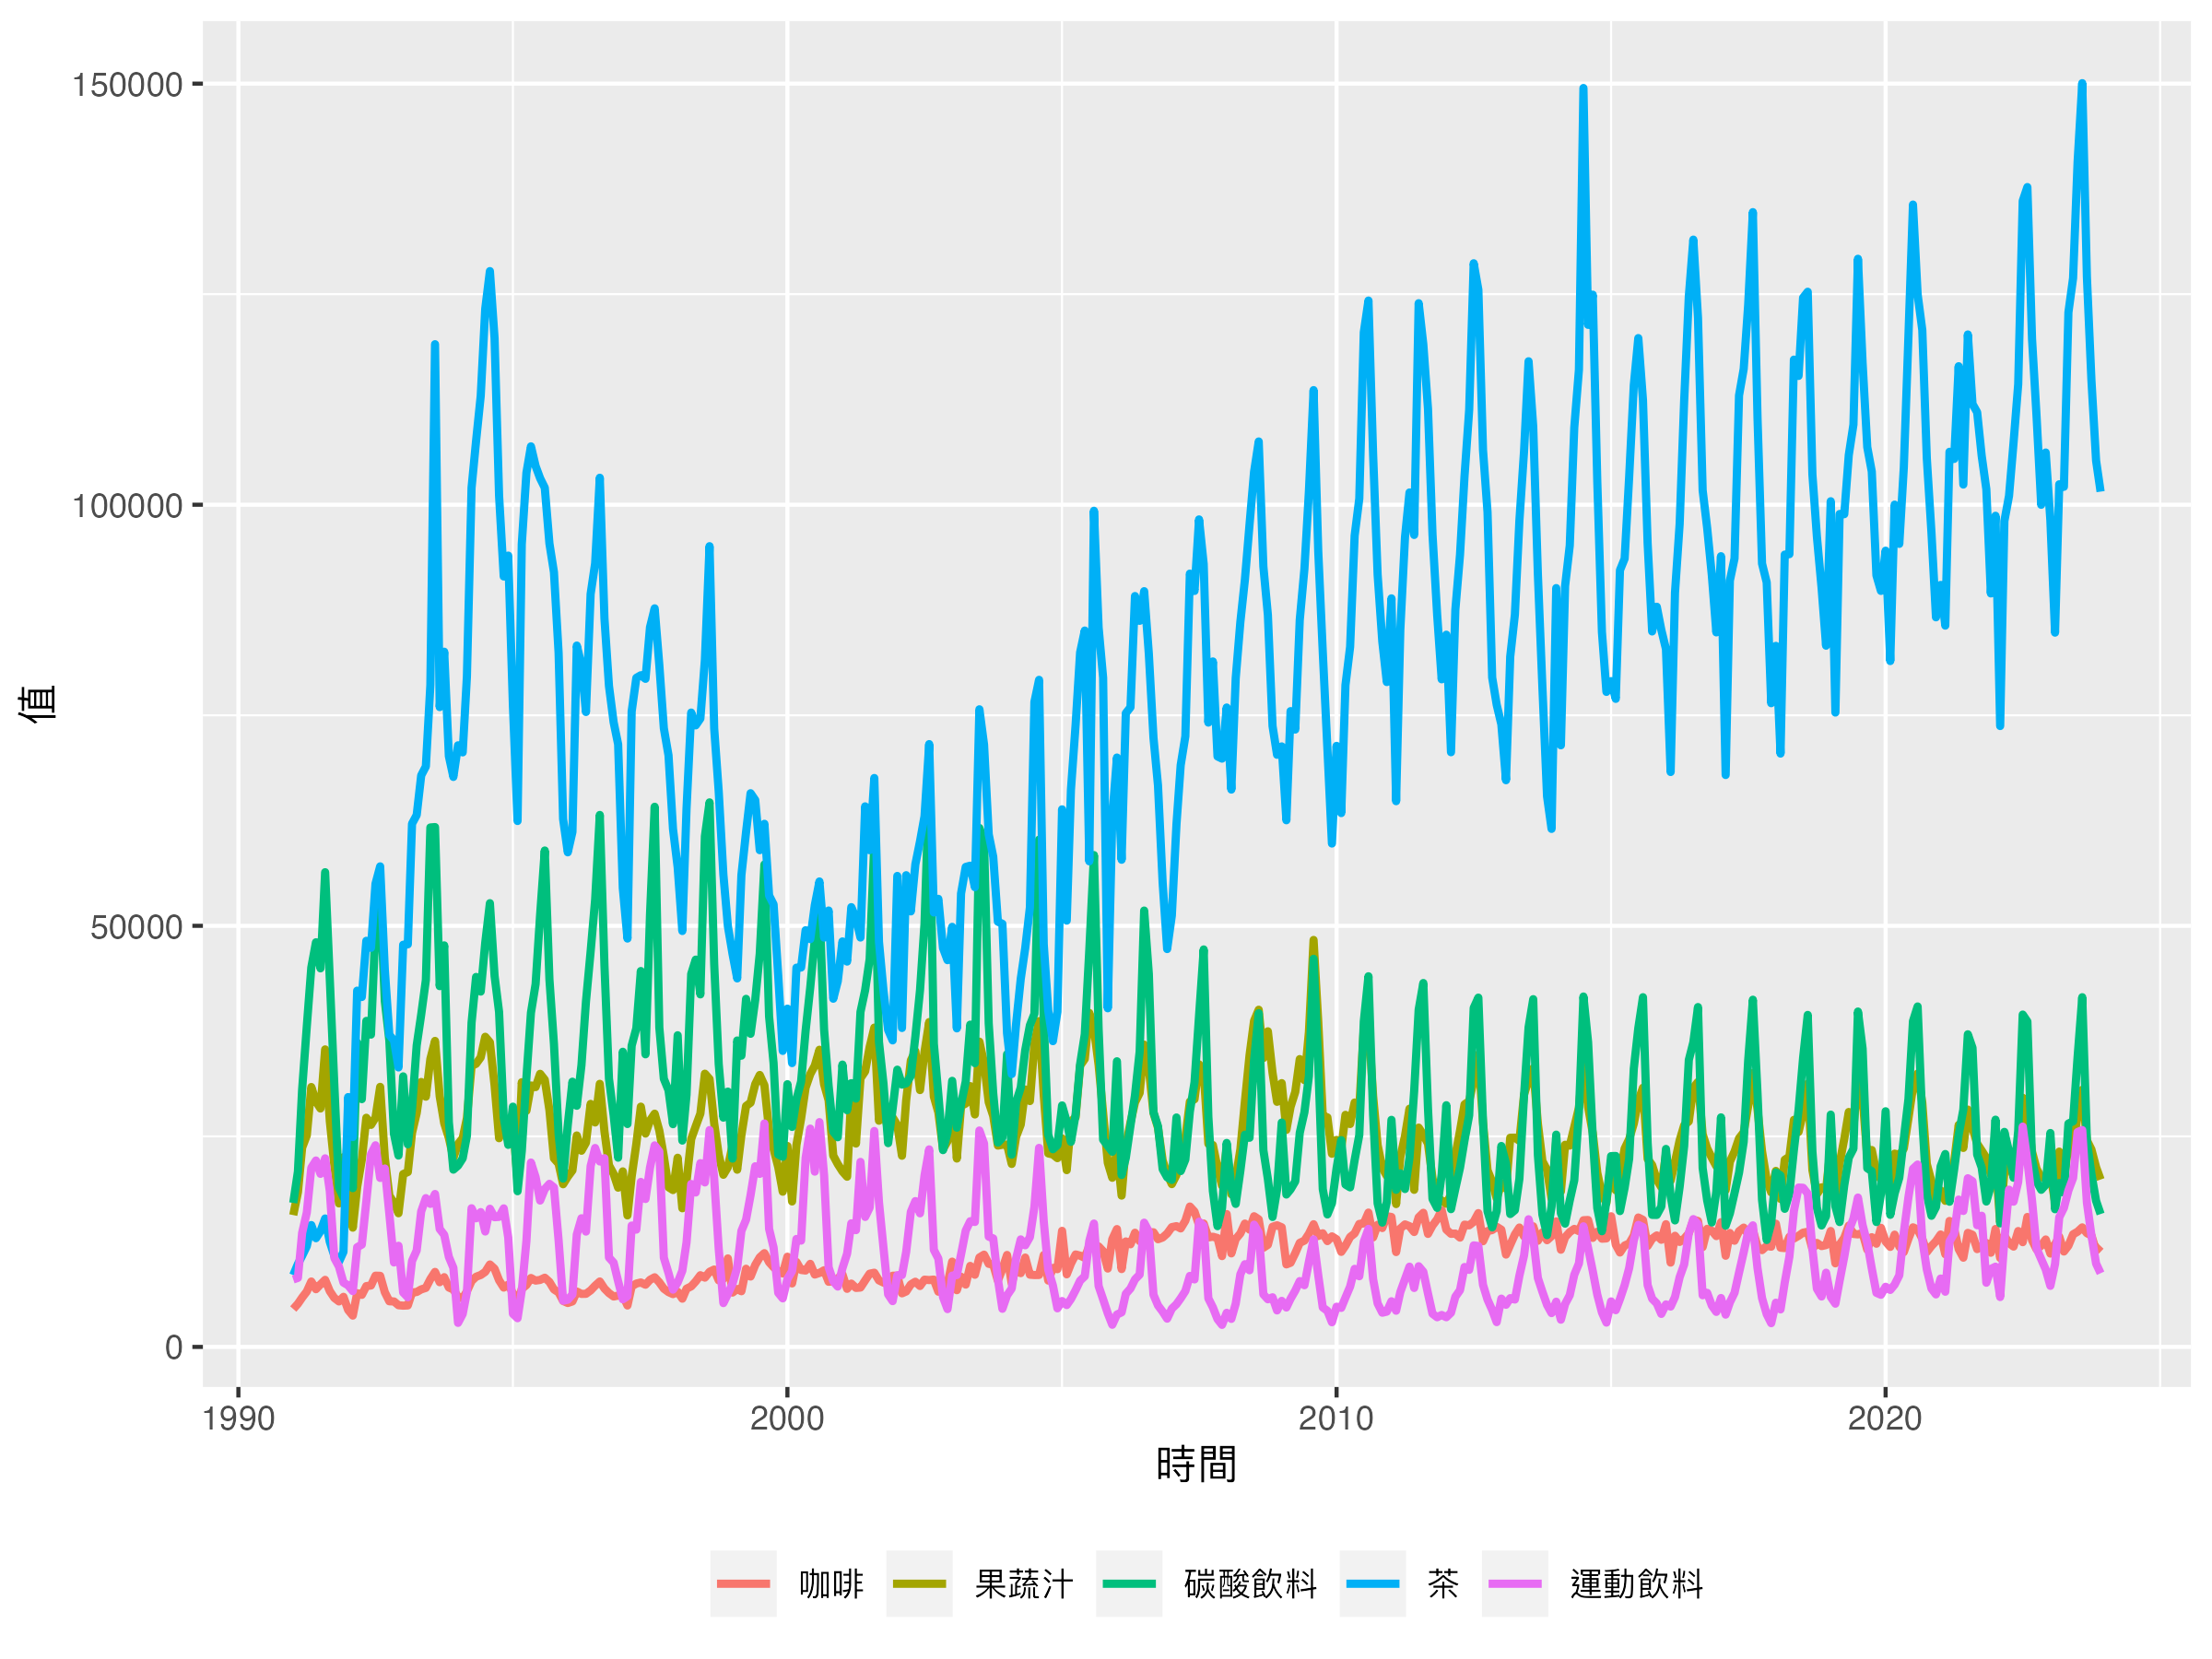
\includegraphics[width=\textwidth]{../outcome/chart1.png}  % both png, jpg can be used for graphs
	 \end{subfigure}
	 \begin{subfigure}[b]{0.65\textwidth}
		\caption{各商品價格時間趨勢} \label{trend_price}
		\vspace{-0.85em}
		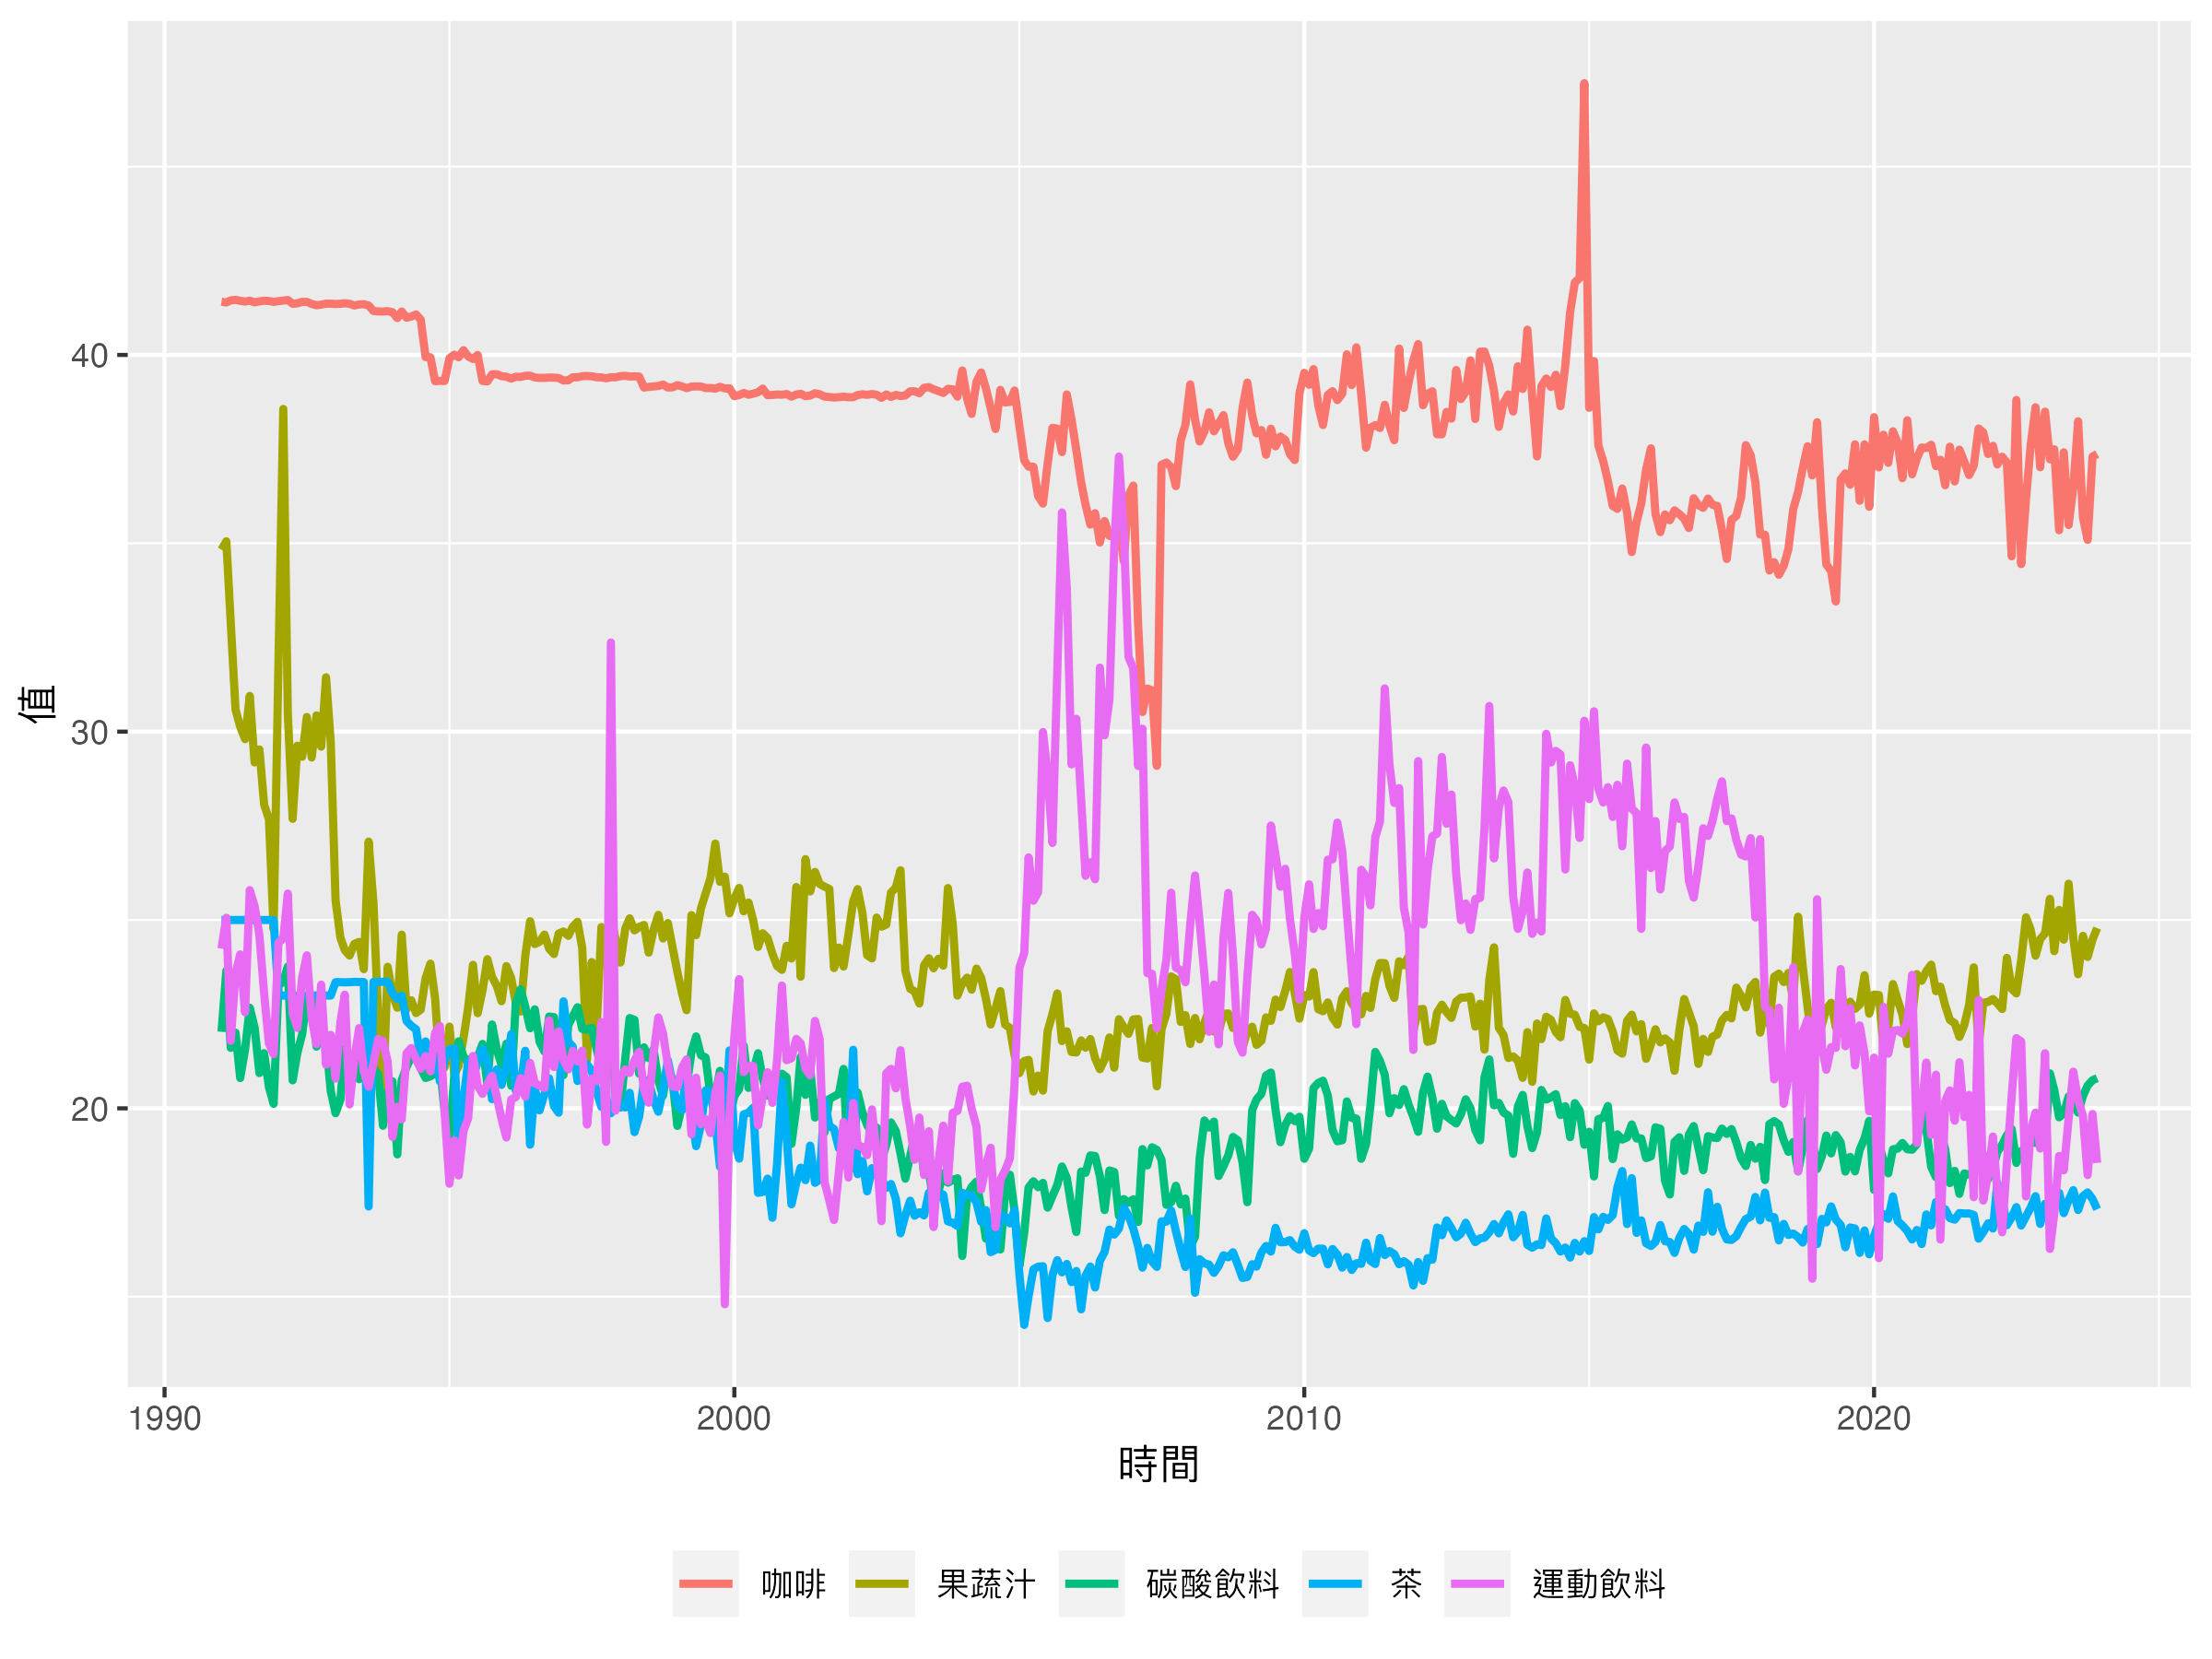
\includegraphics[width=\textwidth]{../outcome/chart2.png}
	\end{subfigure}
\end{center}
\end{figure}
\vspace{-3em}
\begin{singlespace}
        \begin{footnotesize}
        		\noindent {\it Notes:} \ref{trend}為各變數時間變動的趨勢,圖\ref{trend_volume}及圖\ref{trend_price}分別為各商品的銷售量與價格。在銷售量隨時間變化的的圖\ref{trend_volume}中,可以看到明顯的季節性波動,顯示各種飲料在每年都有其週期性,其中可以看到茶的銷售量位居所有飲料之冠。在價格方面,圖 \ref{trend_price}顯示以咖啡的單價最高。
        \end{footnotesize}
\end{singlespace}


\begin{figure}[H]  % [H]固定figure於某一頁
	\begin{center}
	\caption{各變數殘差自相關檢定 (ACF) 分析} \label{ACF}
		\begin{subfigure}[b]{0.65\textwidth}
			 \caption{AIDS模型} \label{ACF_aids}
			\vspace{-0.85em}
			 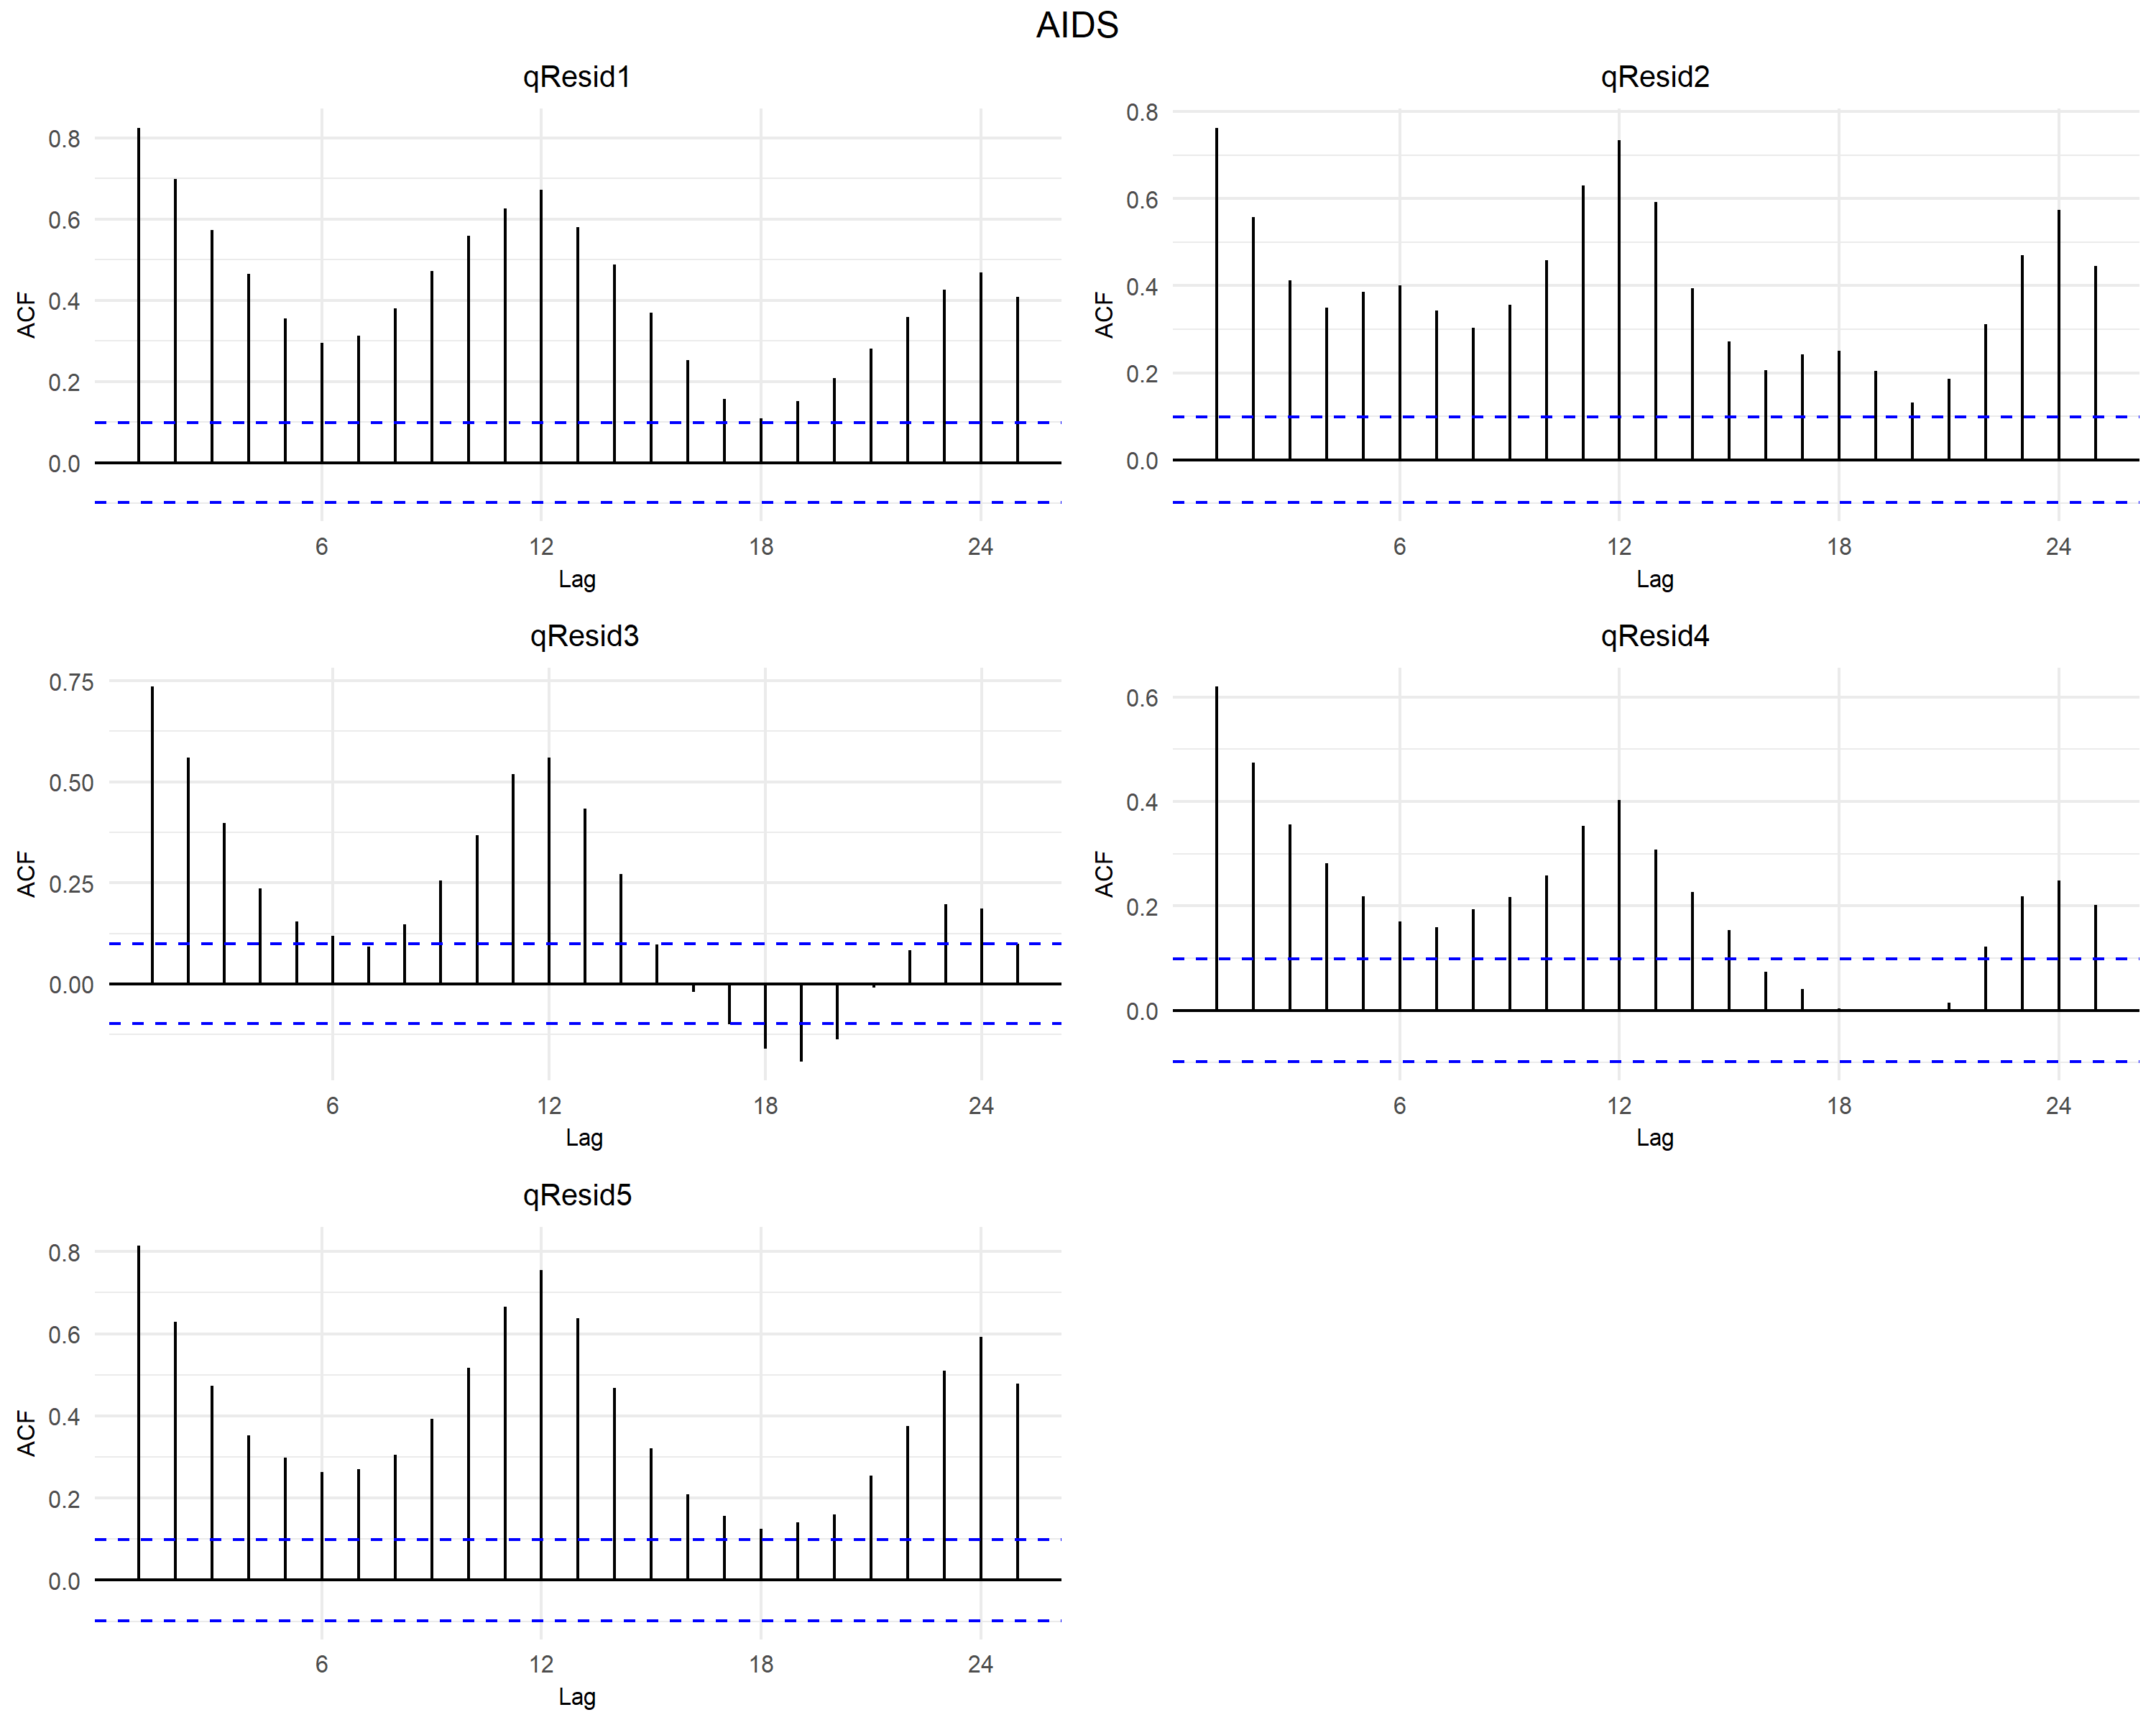
\includegraphics[width=\textwidth]{../outcome/AIDS_plot_qResid.png}  % both png, jpg can be used for graphs
		 \end{subfigure}
		 \begin{subfigure}[b]{0.65\textwidth}
			\caption{LAAIDS模型} \label{ACF_laaids}
			\vspace{-0.85em}
			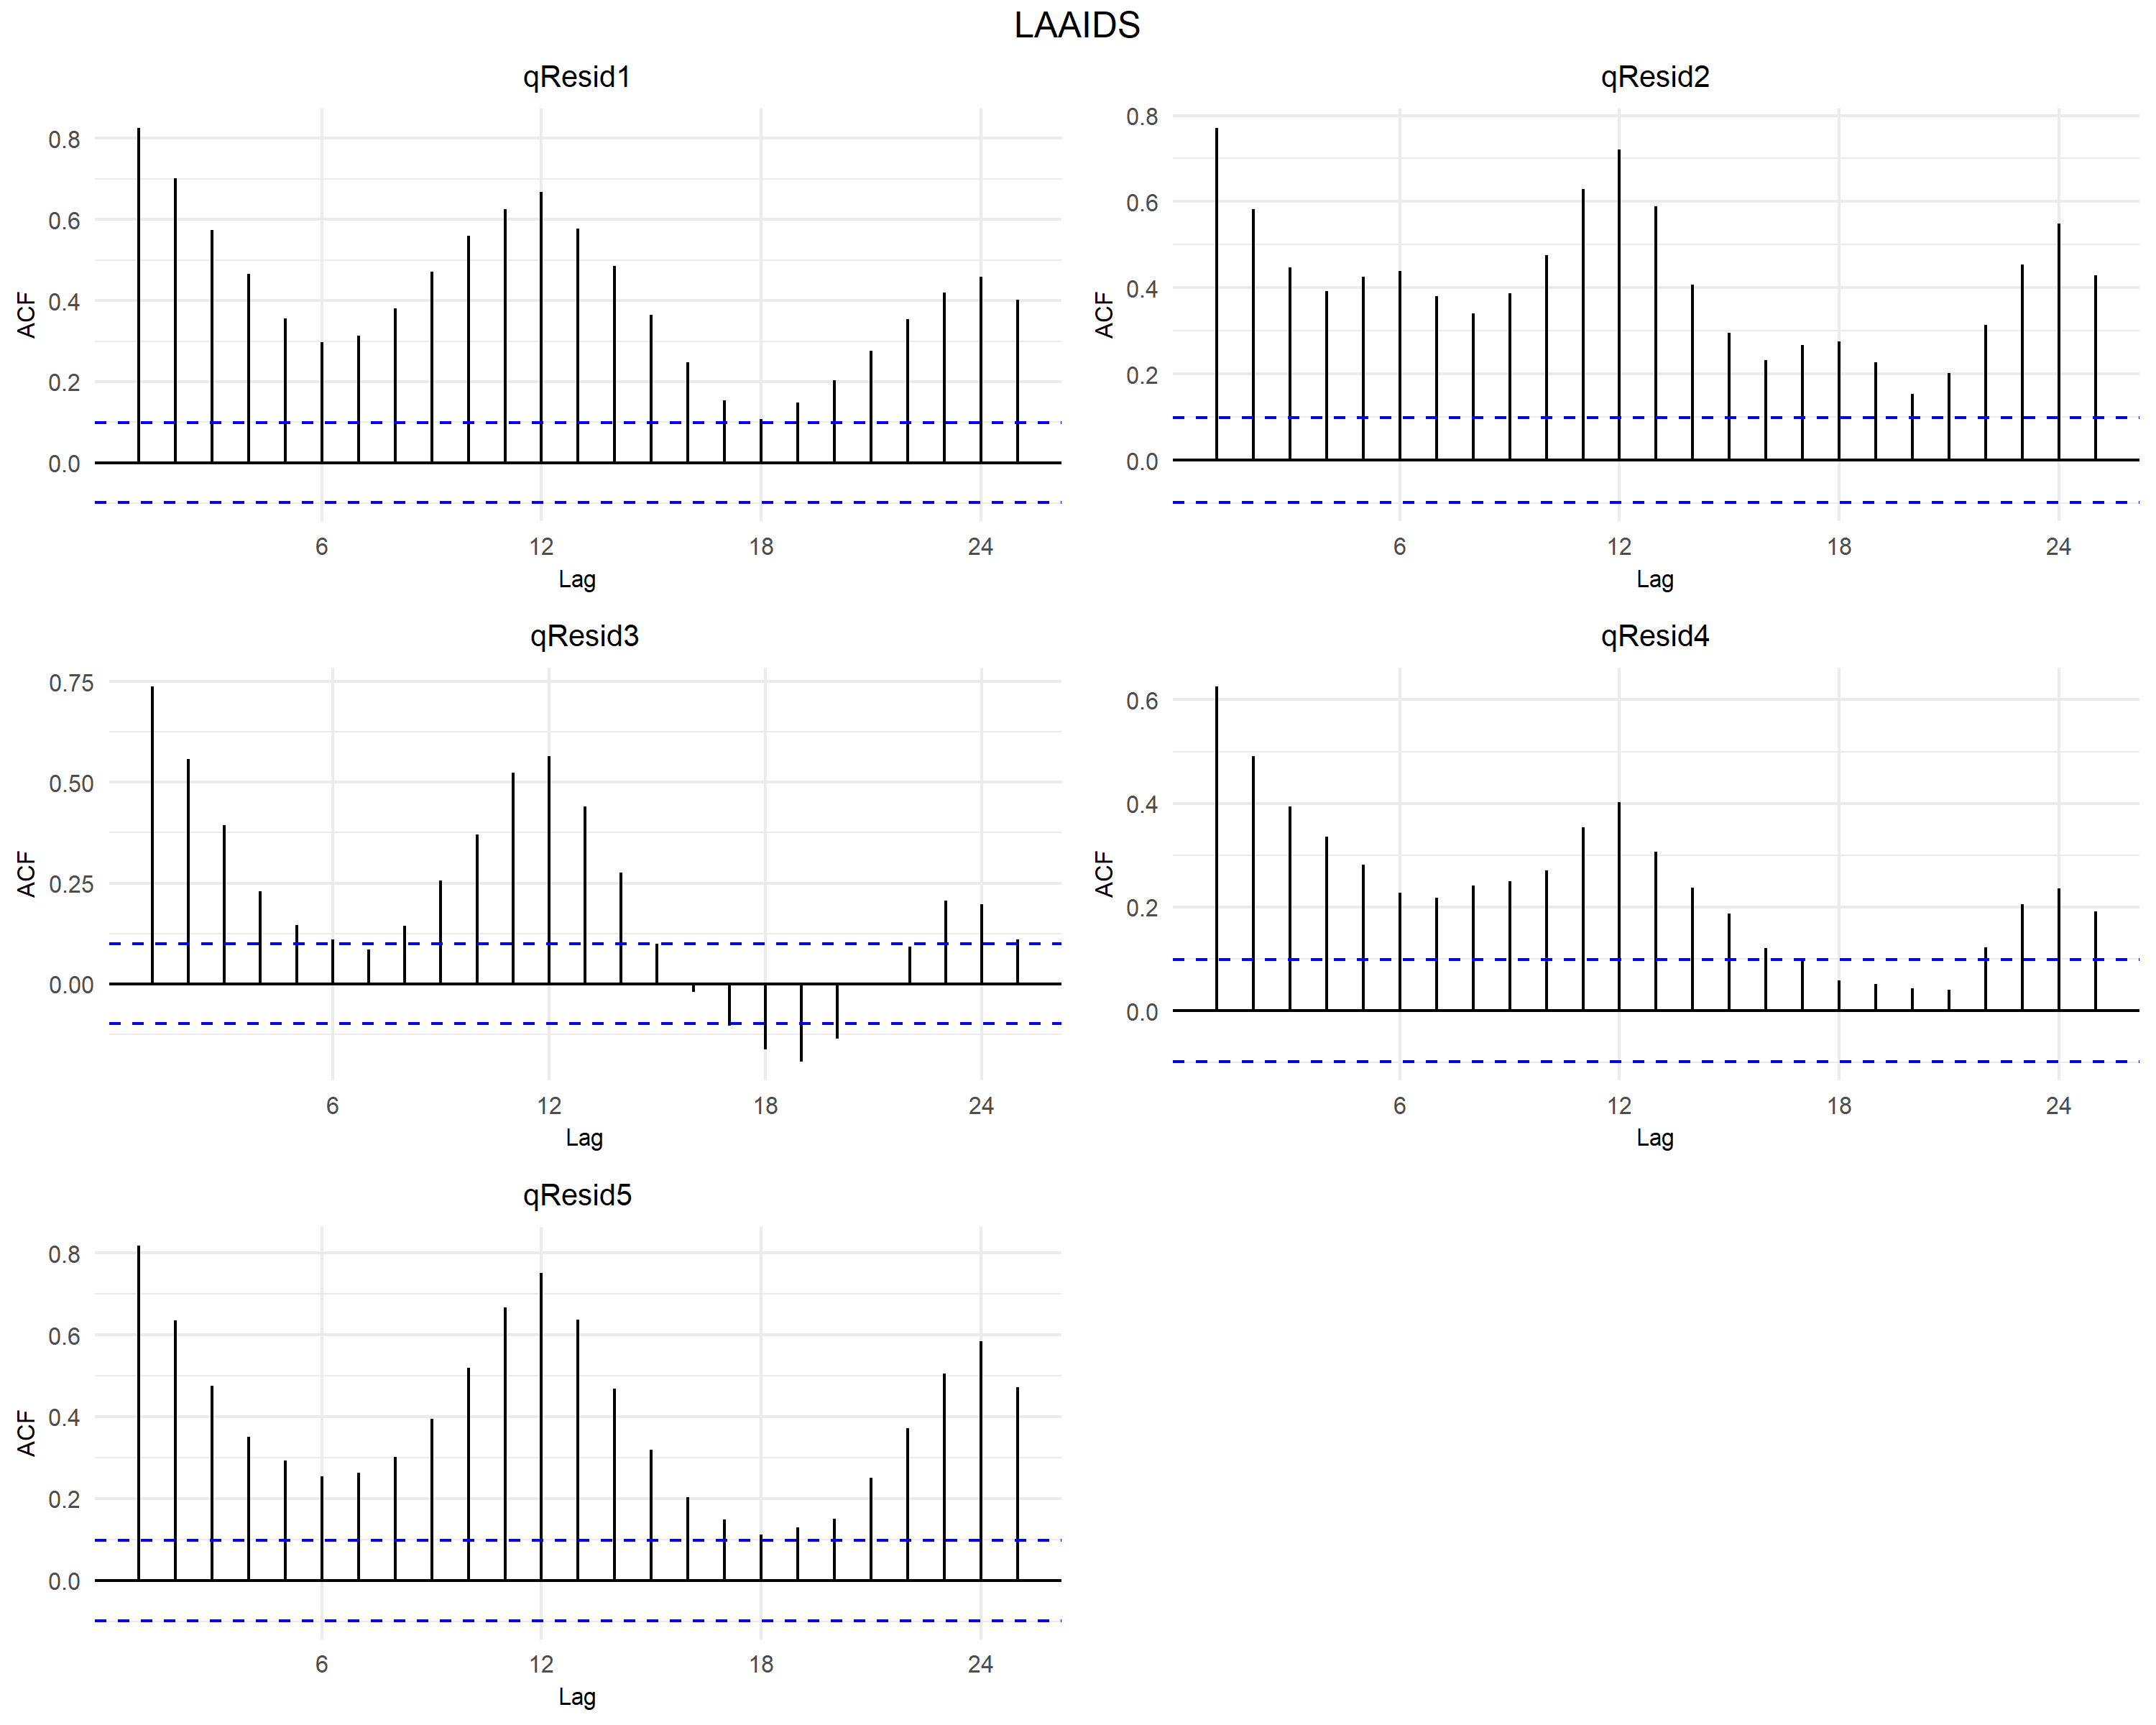
\includegraphics[width=\textwidth]{../outcome/LAAIDS_plot_qResid.png}
		\end{subfigure}
	\end{center}
\end{figure}
\vspace{-3em}
\begin{singlespace}
		\begin{footnotesize}
				\noindent {\it Notes:} qResid1 至 qResid5 分別為果蔬汁、碳酸飲料、運動飲料、咖啡飲料和茶飲料。
				在 AIDS 模型的 ACF 中,果蔬汁、碳酸飲料和茶飲料在低滯後期顯示顯著自相關,且自相關隨滯後增加呈周期性變化,可能與季節性消費相關。
				運動飲料和咖啡飲料在低滯後期的自相關顯著,但隨滯後增加逐漸衰減至不顯著。
				LAAIDS 模型的 ACF 與 AIDS 類似,但碳酸飲料和咖啡飲料的殘差自相關更強。
		\end{footnotesize}
\end{singlespace}



% \newpage
% \begin{figure}[H]
% 	\centering
% 	\caption{The Relationship Between GDP Per Capita and the Total Fertility Rate}\label{fig.gdp_fertility}
% 	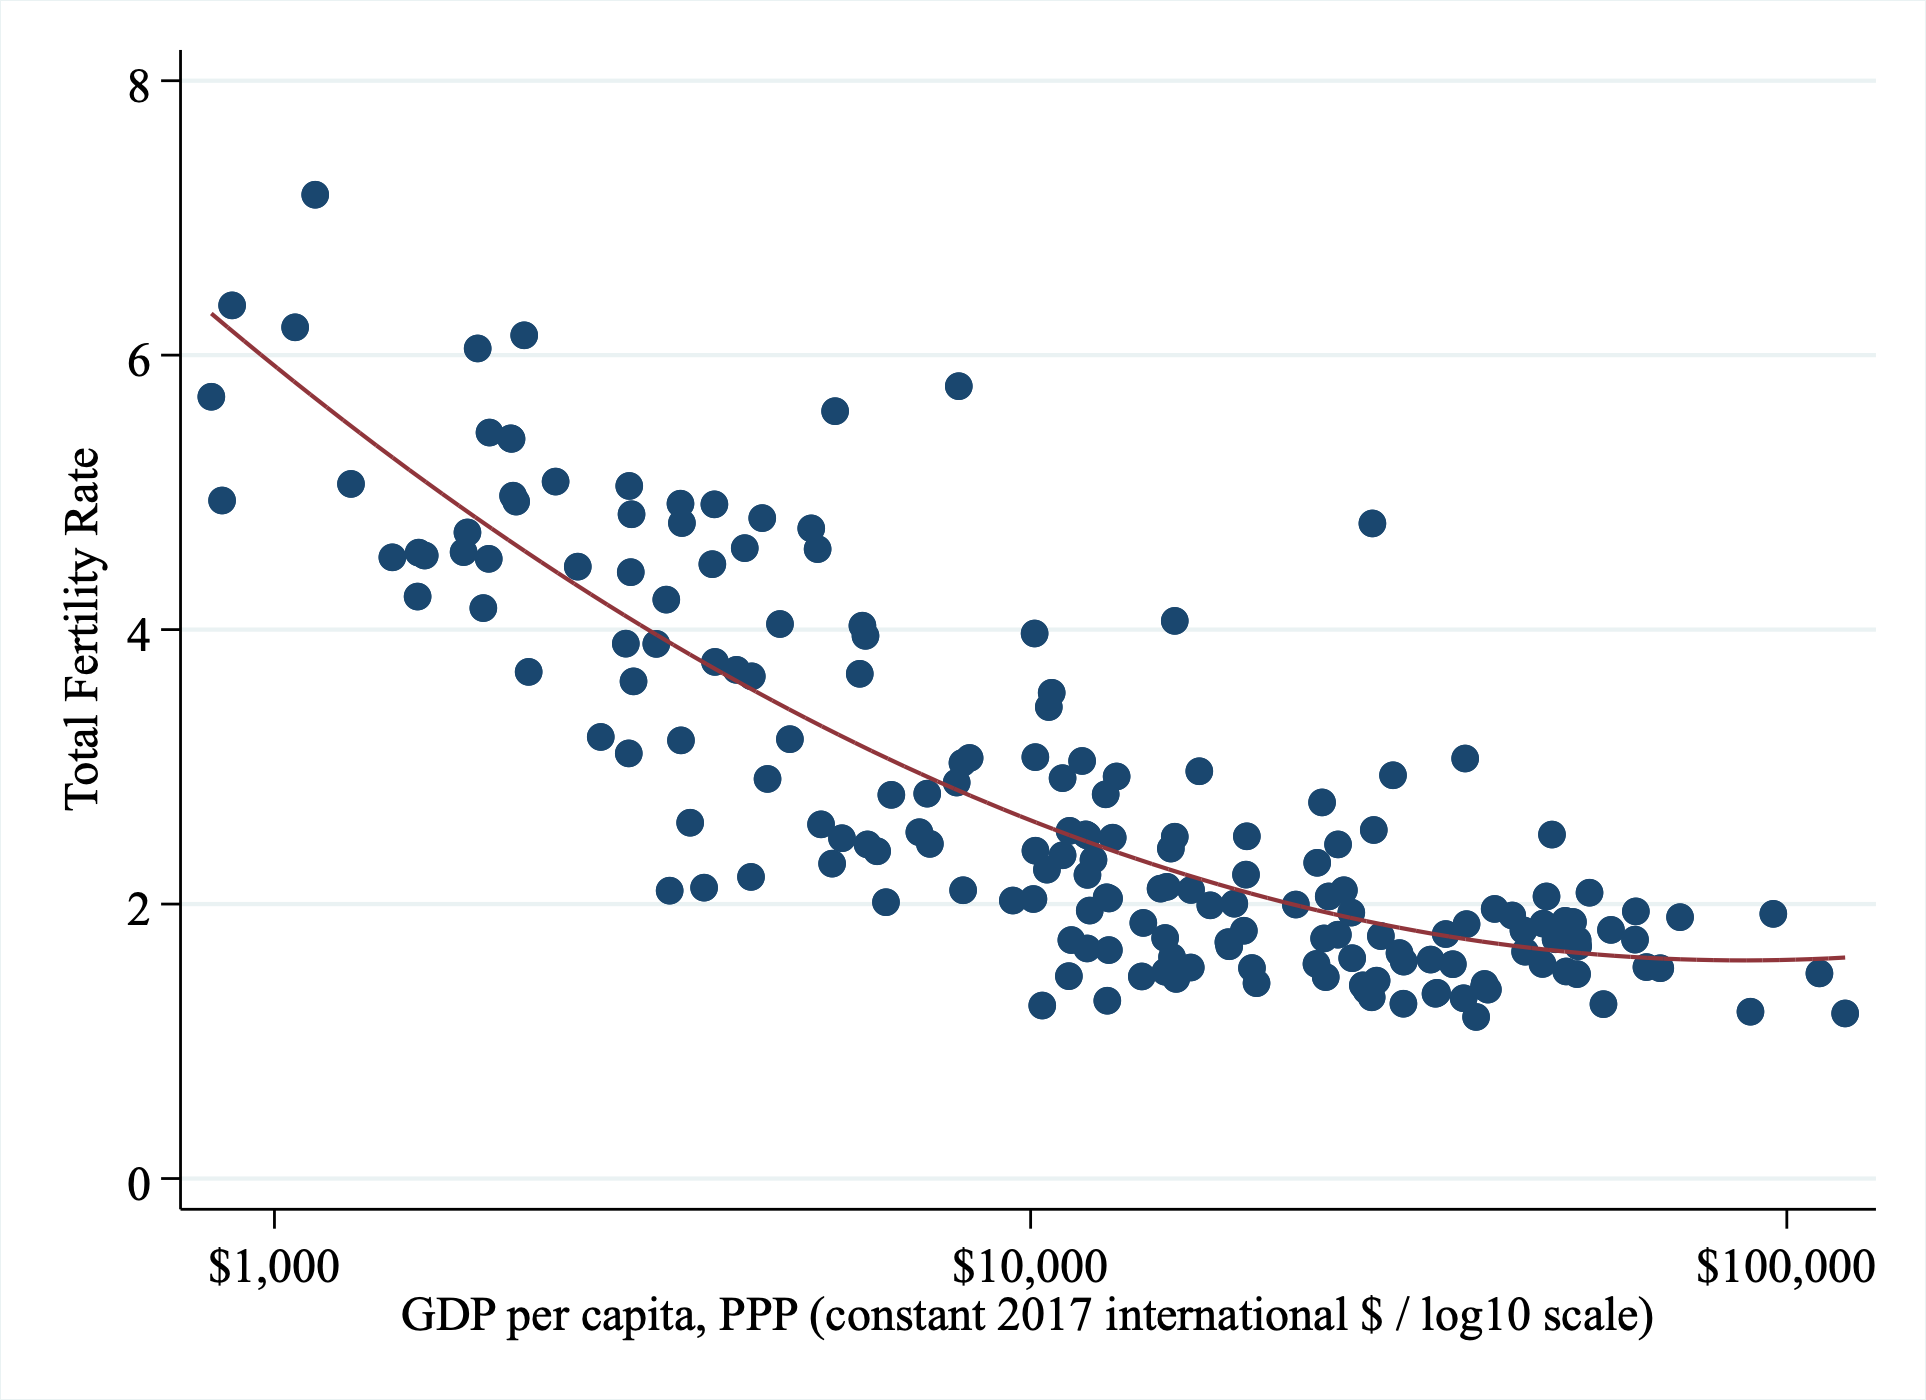
\includegraphics[width=0.8\linewidth]{figures/FC1.jpg}\\
% 	\fontsize{10}{10pt}\selectfont
% 	\flushleft
% 	\emph{Notes:} Each symbol stands for one country. The total fertility rate is defined as the number of children per 1,000 women. The data year is 2020. Data source: Our World in Data \citep{owidfertilityrate,owidgdp}.
% \end{figure}



% \newpage
% \begin{figure}[H]
% 	\centering
% 	\caption{The Relationship Between GDP Per Capita and the Total Fertility Rate}\label{fig.gdp_fertility}
% 	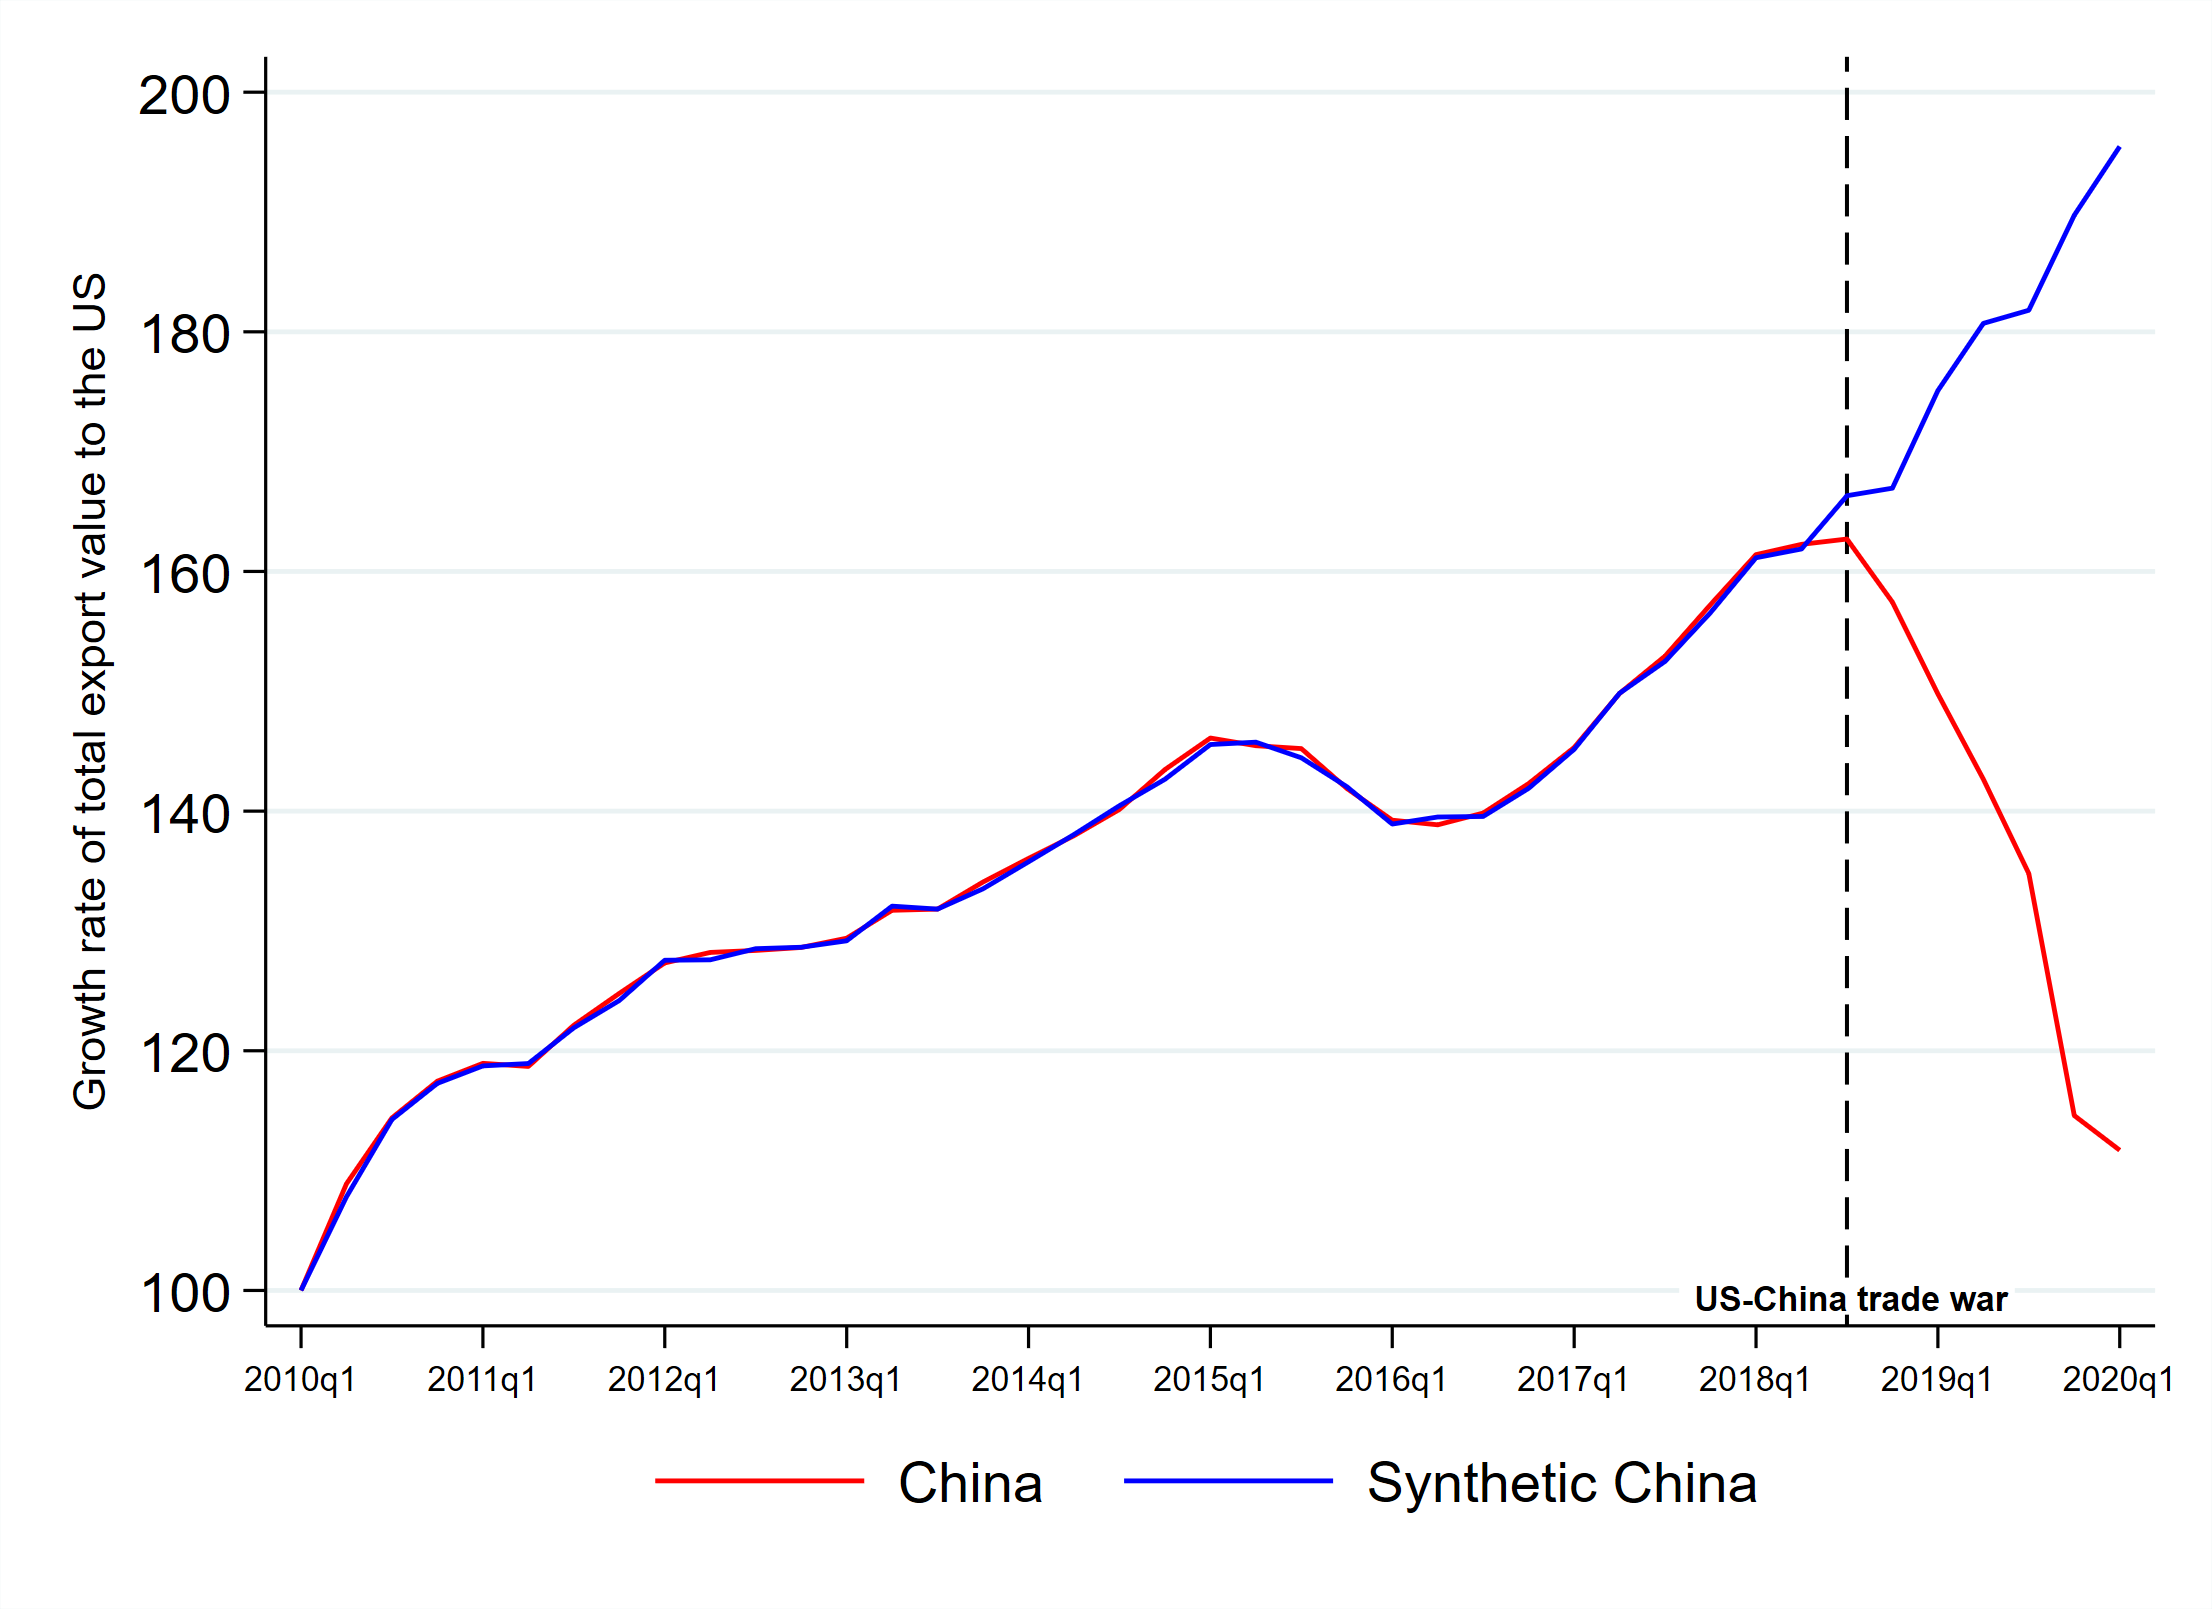
\includegraphics[width=0.8\linewidth]{figures/SCM_us_ch.png}\\
% 	\fontsize{10}{10pt}\selectfont
% 	\flushleft
% 	\emph{Notes:} Each symbol stands for one country. The total fertility rate is defined as the number of children per 1,000 women. The data year is 2020. Data source: Our World in Data \citep{owidfertilityrate,owidgdp}.
% \end{figure}


\end{document}